\chapter{Two-Dimensional Radiative Transfer}\label{Chap:2DRT}
% spell-checker: disable
%TC:group pycode 0 0
\begin{pycode}[2DRT]
name = '2DRT'
ch2DRT = texfigure.Manager(
    pytex,
    './03TwoDRT',
    number=3,
    python_dir='./03TwoDRT/python',
    fig_dir=   './03TwoDRT/Figs',
    data_dir=  './Data/03TwoDRT'
)
\end{pycode}
% spell-checker: enable

% \begin{itemize}
%     \item Adding a dimension to RT, formal solver etc.
%     \item Simulation setup.
%     \item Analysis.
%     \item Suggestions on visibility of this chromospheric glow with DKIST.
% \end{itemize}

It is clear that the world around us is multi-dimensional, but until this point we have only considered radiative transfer in one-dimensional atmospheres.

All of the theory of radiative transfer discussed in previous chapters remains valid when applied to higher dimensional systems, with the exception of the description of the formal solver.
This is due to the non-local terms that appear within the MALI description (with diagonal $\Lambda$ operator) being handled by the formal solver, which is responsible for computing the radiation field throughout the plasma from the local parameters and boundary conditions and thus coupling the atmospheric nodes to each other.
Once the radiation field has been computed it is then used as a local parameter in the rest of the iteration.
In fact, if the storage for the atmosphere is ``flattened'' into a one-dimensional form, the code from the plane-parallel case can (and should) be used to implement the iteration scheme.

In this chapter we shall first describe the extension of the \Lw{} framework to two dimensions (with the possibility of further extension), and then describe its application to the simulation of a flaring atmosphere illuminating an adjacent slab of quiet sun, along with potential implications for future observations at high resolution.

\section{The Formal Solver in Two-Dimensions}

Similarly to the plane-parallel formal solver used in \Lw{}, described previously, we use the short-characteristics method to compute the radiation field throughout the atmosphere.
This approach was first employed in two-dimensions by \citet{Auer1994} using a limited parabolic scheme to avoid overshoot.
We assume the following basis: the $z$-axis is oriented as in the plane-parallel case, oriented vertically from photosphere to corona, the $x$-axis is perpendicular and co-planar to the $z$-axis (in the plane of the page for the following diagrams), and by the right-hand rule the $y$-axis is oriented into the plane of the page.
In the two-dimensional case it is assumed that the atmospheric parameters are homogenous along the $y$-axis, but vary along the $x$- and $z$-axes.
We assume that the atmosphere has a fixed stratification in $x$ and $z$, and that the atmospheric parameters are known at each intersection of these grids.

The mean intensity at each point will be computed similarly to the plane-parallel case; by integration of the local intensity over a weighted angular quadrature.
The Gauss-Legendre nodes used in the plane-parallel case are poorly suited to anisotropy that occurs in the two- and three-dimensional cases, and so we therefore employ the optimised angular quadratures of \citet{Stepan2020} in \Lw{}.

\begin{figure}
\centering
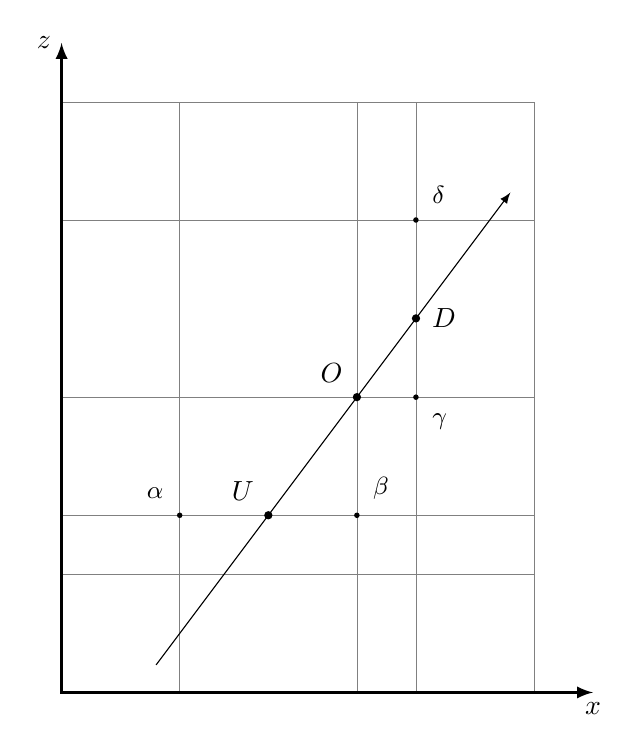
\begin{tikzpicture}[scale=1.5, line width=1pt, >=latex]
    \def\xcoords{1,2,3.5,4,5}
    \def\xmax{5}
    \def\ycoords{1,2,2.5,3.5,5,6}
    \def\ymax{6}
    \def\raym{4/3}
    \def\rayc{-7/6}

    \draw [help lines]
    \foreach \y in \ycoords {
        (1, \y) -- (\xmax, \y)
    }
    \foreach \x in \xcoords {
        (\x, 1) -- (\x, \ymax)
    };
    \draw [<->] ({\xmax+0.5}, 1) node[below] {$x$} -- (1,1) -- (1, {\ymax+0.5}) node[left] {$z$};
    \coordinate (O) at (3.5, 3.5);
    \node[circle, fill=black, inner sep=0 pt, minimum size=3pt, label=above left:{$O$}] at (O) {};
    \draw[->, domain=1.8:4.8, samples=10, thin] plot(\x, {\raym * (\x) + \rayc});
    \coordinate (D) at (4, {\raym * 4 + \rayc});
    \node[circle, fill=black, inner sep=0 pt, minimum size=3pt, label=right:{$D$}] at (D) {};
    \coordinate (U) at ({(2.5 - \rayc) / (\raym)}, 2.5);
    \node[circle, fill=black, inner sep=0 pt, minimum size=3pt, label=above left:{$U$}] at (U) {};

    \node[circle, fill=black, inner sep=0 pt, minimum size=2pt, label={[label distance=0.5mm]above left:{\small $\alpha$}}] at (2, 2.5) {};
    \node[circle, fill=black, inner sep=0 pt, minimum size=2pt, label={[label distance=0.5mm]above right:{\small $\beta$}}] at (3.5, 2.5) {};
    \node[circle, fill=black, inner sep=0 pt, minimum size=2pt, label={[label distance=0.5mm]below right:{\small $\gamma$}}] at (4, 3.5) {};
    \node[circle, fill=black, inner sep=0 pt, minimum size=2pt, label={[label distance=0.5mm]above right:{\small $\delta$}}] at (4, 5) {};
\end{tikzpicture}
\caption{Diagram of short characteristics scheme in two-dimensions.}
\label{Fig:Sc2d}
\end{figure}

For each ray prescribed by the angular quadrature the formal solver must perform one sweep through the grid.
The general case, that of an inclined ray ray travelling through the atmosphere is shown in Fig.~\ref{Fig:Sc2d}.
In the case of this ray the formal solver must sweep first along $x$ and then along $z$.
The difficulties which can arise from this will be discussed in Sec.~\ref{Sec:2dEvalOrder}.
The points $U$ and $D$ refer to them being ``upwind'' and ``downwind'' of the point $O$ for which we are currently computing the intensity.
This can be explained by looking at the intersections of ray with the grid.
To compute the intensity in the direction of this ray at point $O$ using the short characteristics formulation we have, as in one-dimension,
\begin{equation}\label{Eq:MiniScDefinition}
   I_O = I_U e^{-(\tau_U - \tau_O)} + \int_{\tau_O}^{\tau_U} S(t) e^{-(t - \tau_O)}\, dt,
\end{equation}
where these terms have their usual meanings, $I_O$ is the intensity in this direction at $O$, $I_U$ is the intensity in this direction at $U$ and we have dropped the angular and frequency dependencies for clarity.
Thus, to compute the intensity at $O$, the intensity at $U$ must first be known.
As $U$ does not typically lie on a point of our discrete two-dimensional grid, the value of $I_U$ (and other quantities) are not computed directly by the formal solver, and must instead be interpolated from the values of grid points along the line $\alpha\beta$.

Following the short characteristic method, a functional form must be assigned to the variation of $S$ over the the line segment $[UO]$.
In the simplest case, this can again be a linear functional form, but due to the additional dimension for inhomogeneities in the two-dimensional case, unless the grid is very fine or the atmosphere very slowly varying, this may be a poor choice.
A higher order parametrisation of $S$ is likely to require the values of the source function at both $U$ and $D$, and possibly other points along the ray.
Similarly to the cubic Bézier spline method used as standard in our plane-parallel code, we once again turn to monotonic Bézier splines for safe, smooth interpolation, minimising the presence of under and over-shoots.
The cubic method we apply in plane-parallel atmospheres requires four points along $UD$, which becomes less practical in higher dimensions, due to the large computational demands of the method.
Instead we choose the quadratic Bézier spline method, BESSER, of \citet{Stepan2013}, which will be briefly summarised here for the scalar case of the RTE.

\subsection{The BESSER method}

The BESSER method differs from other quadratic Bézier spline methods by ensuring the continuity of the first derivative of the interpolant at $O$.
Due to the large differences in optical depth between adjacent regions (e.g. $\tau_{UO}$ and $\tau_{OD}$) that are likely to occur in multi-dimensional cases with irregular grids, this method is designed so as to guarantee that if the values over $[UOD]$ are monotonic then the spline interpolant will remain monotonic.

The spline interpolant over the $[UO]$ interval is described by
\begin{equation}
    f(a) = (1-a)^2f_U + 2a(1-a)c_U + a^2f_O,\hspace{3em}a\in[0,1],
\end{equation}

where $f_U$ and $f_O$ are the values of $f$ at points $U$ and $O$ respectively, $c_U$ is the functional value of the spline's control point, and $a$ is the normalised coordinate for the distance along $[UO]$.
The control points are points half way along an interval, defining the tangent to the spline at each end of the range i.e. $c_U O$ defines the tangent to the spline at $O$ and $U c_U$ defines the tangent to the spline at $U$.
If we denote the coordinates of our points along the ray $s_U$, $s_O$, and $s_D$ then we have $a = (s - s_U) / h_U$, where $h_U = s_U - s_O$.
An equivalent interpolation can be defined over the $[OD]$ segment.
The monotonicity (for monotonic $f_U$, $f_O$, $f_D$) and continuous first derivative of the interpolating functions at $O$ is ensured by
\begin{enumerate}
    \item Verify the monotonicity of $f_U$, $f_O$, $f_D$, and if $f_O$ is a local extremum then the control points $c_U$ and $c_D$ are set to $f_O$, giving a derivative of zero at $O$. As this is is the only possible solution for this case, the process stops here.

    \item Compute an estimate of the derivative at $O$, by using the derivative of the standard parabolic interpolation of $UOD$.

    \item Use this derivative to compute the initial values at the control points, by direct projection of the first derivative to their coordinates (as this defines a tangent to function at $O$).

    \item Check $c_U \in [f_U, f_O]$. If not, set $c_U$ to $f_U$ to correct for any new extremum and halt the process, as $c_D$ is not needed for the integration of the source function.

    \item Check $c_D \in [f_O, f_D]$. If not, set $c_D$ to $f_D$, and use this to compute a new value for the derivative at $O$, and follow the projection of this tangent to determine $c_U$ (due to the enforced continuity of the derivative at $O$).
\end{enumerate}
This process is described in more detail in \citet{Stepan2013}, but this covers the most important elements of the process.

Similarly to the plane-parallel case, we will solve the RTE in optical depth, due to its increased stability.
This interpolation method can be used to compute $\tau_{UO}$ and $\tau_{OD}$ by
\begin{align}
    \tau_{UO} &= \frac{1}{3}(\chi_U + \chi_O + \chi_{c_U}) (s_O - s_U),\\
    \tau_{OD} &= \frac{1}{2}(\chi_O + \chi_D) (s_D - s_O).
\end{align}
Note that a linear approximation was used for $\tau_{OD}$, as the previous process does not guarantee the calculation of $c_D$.
This could be modified to also use the quadratic spline method, which may be more robust, however the value of $\tau_{OD}$ rarely affects the final solution dramatically.

This method can now be applied to the source function but parametrised along $\tau$ rather than $s$.
The BESSER quadratic spline method is then used to compute the value of the source function control point $S_{c_U}$.
The integral in \eqref{Eq:MiniScDefinition} can now be evaluated, by using the prescribed quadratic spline variation of $S$ over the interval $[\tau_{U}, \tau_{O}]$.
Working through the maths we arrive at
\begin{equation}
    I_D = I_Ue^{-\tau_{UO}} + \omega_U S_U + \omega_O S_O + \omega_{c_U} S_{c_U},
\end{equation}
where,
{
\def\edt{e^{-\tau_{UO}}}
\def\tsq{\tau_{UO}^2}
\begin{align}
    \omega_U &= \frac{2 - (\tsq + 2\tau_{UO} + 2)\edt}{\tsq},\\
    \omega_O &= 2\frac{\tau_{UO} - 2 + \edt (\tau_{UO} + 2)}{\tsq},\\
    \omega_{c_U} &= 1 - 2 \frac{\edt + \tau_{UO} - 1}{\tsq}.
\end{align}
}

For small values of $\tau_{UO}$ the numerical precision of the exponential function becomes unreliable (in floating point arithmetic), so for this reason these are replaced with Taylor expansions for $\tau_{UO}\lesssim 0.1$.

An expression for the $\Lambda^*$ operator can then be devised equivalently to the process used previously for the plane-parallel case.
The source function is locally set to unity, and zero elsewhere.
This implies that $c_U$ is also set to 1.
Thus the local contribution to the radiation field is given by
\begin{equation}
    \Lambda^*(\nu, \vec{d}) = \omega_{c_U} + \omega_O,
\end{equation}
and remains related to $\Psi^*$ by the local opacity.

The equivalent integration and $\Lambda$ operator coefficients for a linear short characteristics approach can be computed similarly and are analogous to those computed in the one-dimensional case.

\subsection{Evaluation Order and Boundary Conditions}\label{Sec:2dEvalOrder}

Looking more closely at the order in which the formal solver needs to sweep the grid, we can see that the point $O$ for the ray discussed in the previous section (and shown in Fig.~\ref{Fig:Sc2d}) would be the 10th node to be solved, and this ordering is shown in Fig.~\ref{Fig:2DSweep}.
Most of the nodes on this figure are solved equivalently to this one, with all necessary quantities known at evaluation time provided the sweep order is preserved, but there are several question marks which require explanation.

\begin{figure}
\centering
\subimport{03TwoDRT/}{SweepOrder}
\caption{Diagram of sweep order in 2D}
\label{Fig:2DSweep}
\end{figure}

The {\color{TolBlue} blue} question marks along the $x$ axis all require values that must be computed from the boundary conditions.
The upper and lower boundary conditions in $z$ are typically taken to be described by a defined in-going radiation field (possibly zero or based on a black body).
The upper and lower boundaries in $x$ can be described by fixed boundary conditions, but it is also common to describe these with periodic boundary conditions where the ray wraps from one side of the grid to the other.
The {\color{TolTeal} teal} question marks along the upper $x$ boundary can then be interpreted in multiple ways; in the case of periodic boundary conditions they can be prolonged along the {\color{TolTeal} teal} arrows, and used in the same way as the previously described case.
If fixed boundary conditions are used then the intensity at these points must be computed by a linear formal solver indicated by the black arrows ending at the nodes labelled 4 and 8.

Finally, the region around the {\color{TolOrange} orange} question mark, the tail end of the arrow passing through node 11, requires some additional explanation.
In the configuration shown here, the arrow can stop at its intersection with the vertical line on which nodes 6 and 10 lie as the intensity information has been computed at both of these.
If an equivalent situation occurs at a periodic $x$ boundary, then a long characteristics approach will need to be applied to this ray.
This implies that the ray will need to be prolonged back to the previous intersection with a horizontal grid line, where the necessary intensity values can be interpolated, as is shown on this figure.
There are multiple options for treating the integration over the segment between this upwind point and the node.
Whilst it is possible to take this segment as a singular integration term, very inclined rays may cross multiple vertical grid lines and regions with dramatically varying parameters.
For this reason it is common to sub-step along this ray, performing an accumulated short-characteristics integration along each subinterval.

Another problem that may arise, closely related to choosing the correct upwind point, is that of velocity shifts in the medium.
\citet{VanNoort2002} discussed the possibility of the opacity over an integration integral being underestimated due to differing Doppler shifts at each end of the segment affecting the local opacity by a large margin (say from the core to the wing of the line).
As commented by \citet{Ibgui2013}, it is also possible for this effect to overestimate the opacity along this segment, in a similar manner.
The most common solution to this, proposed by \citet{VanNoort2002}, and explained in detail in \citet{Ibgui2013} is to subgrid along the ray.
The ray is then divided into subintervals along which the velocity may only change by a small (implementation defined) amount relative to the thermal velocity.
This approach can be very expensive when large Doppler shifts are present, due to the work involved in computing these segments, interpolating the necessary parameters to each start/end point (this will now require interpolation on both axes, rather than simply one as in the basic case discussed thus far), and the extra numerical integration steps.
This subgridding technique is not currently supported in \Lw{} but the code was designed with this method in mind, and a sensible location has been left for its implementation.

\subsection{Implementation Details}

The restrictive ordering of a formal solver sweep discussed in the previous section imposes constraints on the parallelisation of this algorithm.
% In the case of a single-threaded program, it is sufficient to obey this order, however, when distributing work across threads or multiple computing nodes it is essential that the necessary information be present to avoid computation stalls, or the use of uninitialised data.
There is an in-depth discussion of an advanced spatial and frequency parallelisation algorithm for multi-dimensional radiative transfer in \citet{Stepan2013}, however in \Lw{} we assume that the entire simulation domain can be held in memory and the formal solver is parallelised in frequency, equivalently to the plane-parallel case.

The data structures for storing the atmospheric and population information in \Lw{} were updated to support two dimensional atmospheres, storing the data contiguously so as to be able to reuse the core iteration machinery from the plane-parallel case (as inspired by the RH code).
Two-dimensional formal solvers can be loaded from external libraries via the same interface as used for their one-dimensional counterparts, and through these interfaces we ensure the modularity of \Lw{}.
An equivalent interface is also defined for the interpolation function to be used in two-dimensions, giving flexibility in the interpolation order and any form of limiting used (which may need to be adapted to specific grids).
\Lw{} provides default implementations of the two-dimensional linear and BESSER short-characteristics formal solvers, along with linear and BESSER interpolation schemes for the necessary parameters.
The framework defaults to the BESSER formal solver with linear interpolation for the parameters.

For efficiency, the calculation of the ray-grid intersections is performed in a separate pre-pass to the formal solution, as this information can be reused for each formal solution using the same angular quadrature.
Whilst it is possible to compute the necessary parameter interpolation weights at this stage, we choose not to do this, as it would render the interpolation interface either more limited, or substantially more complex, due to the need to utilise different numbers of interpolation weights for different schemes.
We instead opt to store fractional indices which can be used in conjunction with the grid information in any interpolation procedure.
Using 64-bit arithmetic these are a concise and robust method for storing these locations.
By design, the intersection calculation is only performed for one upwind and downwind point
(excluding long characteristics that cross grid boundaries), as the second order method is considered to be a sufficient trade-off in terms of computational cost against accuracy.
This could easily be updated in the future, and we acknowledge that this is a limitation in terms of the two-dimensional formal solvers that can be loaded via the external interface.


\subsection{Validation}

\setpythontexautoprint{false}
% spell-checker: disable
\begin{pycode}[2DValidation]
# NOTE(cmo): Hack to minimise the number of times this session needs to be run
ch2DRT = texfigure.Manager(
    pytex,
    './03TwoDRT',
    number=3,
    python_dir='./03TwoDRT/python',
    fig_dir=   './03TwoDRT/Figs',
    data_dir=  './03TwoDRT/Data'
)

# def data_file_path(manager, fileName):
#     return os.path.join(manager.data_dir, fileName)

# twoDFilename = '2DPlotData.pickle'
# try:
#     with pickle.open(ch2DRT.data_file(twoDFilename), 'rb') as f:
#         data2d = pickle.load(f)
# except:
from lightweaver.fal import Falc82
from lightweaver.rh_atoms import H_6_atom, H_6_CRD_atom, H_3_atom, C_atom, O_atom, OI_ord_atom, Si_atom, Al_atom, CaII_atom, Fe_atom, FeI_atom, He_9_atom, He_atom, He_large_atom, MgII_atom, Mg_atom, N_atom, Na_atom, S_atom
import lightweaver as lw
import matplotlib.pyplot as plt
import time
import pickle
import numpy as np
from lightweaver.utils import NgOptions, get_default_molecule_path
from lightweaver.LwCompiled import FastBackground

atmos1d = Falc82()
atmos1d.quadrature(5)
x = (np.arange(5) * 5_000).astype(np.float64)
Nx = x.shape[0]
z = np.copy(atmos1d.height)
Nz = z.shape[0]
temperature = np.zeros((Nz, Nx))
temperature[...] = atmos1d.temperature[:, None]
vx = np.zeros((Nz, Nx))
vz = np.zeros((Nz, Nx))
vturb = np.zeros((Nz, Nx))
vturb[...] = atmos1d.vturb[:, None]
ne = np.zeros((Nz, Nx))
ne[...] = atmos1d.ne[:, None]
nHTot = np.zeros((Nz, Nx))
nHTot[...] = atmos1d.nHTot[:, None]
atmos = lw.Atmosphere.make_2d(height=z, x=x, temperature=temperature, vx=vx, vz=vz, vturb=vturb, ne=ne, nHTot=nHTot)
atmos.quadrature(6)

wave = np.linspace(853.9444, 854.9444, 501)
rayDir = 0.9

aSet = lw.RadiativeSet([H_6_atom(), C_atom(), O_atom(), Si_atom(), Al_atom(), CaII_atom(), Fe_atom(), He_atom(), Mg_atom(), N_atom(), Na_atom(), S_atom()])
aSet.set_active('Ca')
spect = aSet.compute_wavelength_grid()

eqPops1d = aSet.compute_eq_pops(atmos1d)
ctx1d = lw.Context(atmos1d, spect, eqPops1d, Nthreads=16, conserveCharge=False)

# dPopsStop = [1e-1, 1e-2, 1e-3, 1e-4]
dPopsStop = np.logspace(-1, -4, 10)
Iwave1ds = []
Iwaves = []

start1d = time.time()
for i in range(2):
    ctx1d.formal_sol_gamma_matrices()
dPops = [1.0]
currentStop = 0
for i in range(2000):
    ctx1d.formal_sol_gamma_matrices(lambdaIterate=False)
    dPops.append(ctx1d.stat_equil())
    if dPops[-1] < dPopsStop[currentStop]:
        Iwave1d = ctx1d.compute_rays(wave, rayDir)
        Iwave1ds.append(Iwave1d)
        currentStop += 1
    if dPops[-1] < 1e-4:
        print(i)
        break
end1d = time.time()
time1d = end1d - start1d
Niter1d = i

eqPops = aSet.compute_eq_pops(atmos)
start = time.time()
bgProvider = lambda *args: FastBackground(*args, Nthreads=16)
ctx = lw.Context(atmos, spect, eqPops, Nthreads=16, conserveCharge=False, backgroundProvider=bgProvider)

start = time.time()
for i in range(2):
    ctx.formal_sol_gamma_matrices()
dPops = [1.0]
currentStop = 0
for i in range(2000):
    ctx.formal_sol_gamma_matrices(lambdaIterate=False)
    dPops.append(ctx.stat_equil())
    if dPops[-1] < dPopsStop[currentStop]:
        Iwave = ctx.compute_rays(wave, rayDir)
        Iwaves.append(Iwave)
        currentStop += 1
    if dPops[-1] < 1e-4:
        print(i)
        break
end = time.time()
time2d = end - start
Niter2d = i

wave = np.linspace(853.9444, 854.9444, 501)
wave -= CaII_atom().lines[-1].lambda0
\end{pycode}

\begin{pycode}[2DValidation]
fig, ax = plt.subplots(2, 1, figsize=texfigure.figsize(pytex, scale=1, height_ratio=0.8))
ax[0].plot(wave, Iwave1d, label=r'1D Reference')
ax[0].set_xlim(wave[0], wave[-1])
for j in range(ctx.spect.I.shape[-1]):
    ax[0].plot(wave, Iwave[:, j], '--', label=('2D, $x={:.0f}$\,\si{{\kilo\metre}}'.format(atmos.x[j] / 1e3)))
ax[0].legend()
ax[0].set_ylabel(r'Specific Intensity [SI]')
ax[0].set_xlim(wave[0], wave[-1])

ax[1].plot(wave, (Iwave[:, 2] - Iwave1d) / Iwave[:, 2])
ax[1].set_xlabel(r'$\Delta\lambda$ [\si{\nano\metre}]')
ax[1].set_ylabel(r'Relative Error')
ax[1].set_xlim(wave[0], wave[-1])
lFig = ch2DRT.save_figure('2DValidation', fig, fext='.pgf')
lFig.caption = r'Validation of 2D formal solver in static FALC atmosphere with periodic $x$ boundary conditions.'
\end{pycode}

\begin{pycode}[2DValidation]
fig = plt.figure(figsize=texfigure.figsize(pytex, scale=1, height_ratio=0.7))
ax = plt.gca()

maxChanges = []
l2s = []

def l2_norm(x, y):
    return np.mean((x - y)**2)

for i in range(len(Iwaves)):
    maxChanges.append(np.max(np.abs(Iwaves[i][:, 2] - Iwave1ds[i])))
    l2s.append(l2_norm(Iwaves[i][:, 2], Iwave1ds[i]))

ax.plot(dPopsStop, maxChanges, '+-', label='Max Difference')
ax.invert_xaxis()
ax1 = ax.twinx()
ax1.plot(dPopsStop, l2s, '+-', label='L2 Norm', c='C1')
# ax.legend()
ax.set_xscale('log')
ax.set_yscale('log')
ax1.set_yscale('log')
ax.set_xlabel(r'$\mathrm{max}(\Delta n / n)$')
ax.set_ylabel(r'Absolute Maximum Difference', c='C0')
ax1.set_ylabel(r'L2 Norm', c='C1')

lFig = ch2DRT.save_figure('2DErrChange', fig, fext='.pgf')
lFig.caption = r'Standard convergence metric (absolute maximum difference) and L2 difference of the \CaLine{} line profiles between between the 1 and 2D Formal Solvers (including ALI iteration procedure).'
\end{pycode}

\begin{pycode}[2DValidation]
from copy import copy
from weno4 import weno4

atmos1d = Falc82()
atmos1d.vlos[:] = -np.sin(atmos1d.height / atmos1d.height[0] * 2 * np.pi) * 20e3
atmos1d.vlos[-3:] = 0.0
atmos1d.vlos[:3] = 0.0
atmos1d.quadrature(5)
x = (np.arange(5) * 5_000).astype(np.float64)
Nx = x.shape[0]
z = np.copy(atmos1d.height)
Nz = z.shape[0]
temperature = np.zeros((Nz, Nx))
temperature[...] = atmos1d.temperature[:, None]
vx = np.zeros((Nz, Nx))
vz = np.zeros((Nz, Nx))
vz[...] = atmos1d.vlos[:, None]
vturb = np.zeros((Nz, Nx))
vturb[...] = atmos1d.vturb[:, None]
ne = np.zeros((Nz, Nx))
ne[...] = atmos1d.ne[:, None]
nHTot = np.zeros((Nz, Nx))
nHTot[...] = atmos1d.nHTot[:, None]
atmos = lw.Atmosphere.make_2d(height=z, x=x, temperature=temperature, vx=vx, vz=vz, vturb=vturb, ne=ne, nHTot=nHTot)
atmos.quadrature(6)

wave = np.linspace(853.9444, 854.9444, 501)
rayDir = 0.9

aSet = lw.RadiativeSet([H_6_atom(), C_atom(), O_atom(), Si_atom(), Al_atom(), CaII_atom(), Fe_atom(), He_atom(), Mg_atom(), N_atom(), Na_atom(), S_atom()])
aSet.set_active('Ca')
spect = aSet.compute_wavelength_grid()

eqPops1d = aSet.compute_eq_pops(atmos1d)
ctx1d = lw.Context(atmos1d, spect, eqPops1d, Nthreads=16, conserveCharge=False)


for i in range(2):
    ctx1d.formal_sol_gamma_matrices()
dPops = [1.0]
for i in range(2000):
    ctx1d.formal_sol_gamma_matrices(lambdaIterate=False)
    dPops.append(ctx1d.stat_equil())
    if dPops[-1] < 1e-4:
        print(i)
        break

eqPops = aSet.compute_eq_pops(atmos)
start = time.time()
bgProvider = lambda *args: FastBackground(*args, Nthreads=16)
ctx = lw.Context(atmos, spect, eqPops, Nthreads=16, conserveCharge=False, backgroundProvider=bgProvider)

for i in range(2):
    ctx.formal_sol_gamma_matrices()
dPops = [1.0]
currentStop = 0
for i in range(2000):
    ctx.formal_sol_gamma_matrices(lambdaIterate=False)
    dPops.append(ctx.stat_equil())
    if dPops[-1] < 1e-4:
        print(i)
        break

IwaveVlos = ctx.compute_rays(wave, rayDir)
Iwave1dVlos = ctx1d.compute_rays(wave, rayDir)


class FixedXBc(lw.BoundaryCondition):
    def __init__(self, ctx1d):
        self.ctx1d = ctx1d
        self.I = None
        self.Nrays = 0
        self.anglesDirty = False
        self.muz = None

    def set_bc(self, I1d):
        self.I = I1d.reshape(I1d.shape[0], -1, I1d.shape[-1])

    def set_required_angles(self, mux, muy, muz, indexVector):
        if self.muz is None \
           or self.muz.shape[0] != muz.shape[0] \
           or np.any(self.muz != muz):
            self.anglesDirty = True
        return super().set_required_angles(mux, muy, muz, indexVector)

    def compute_bc(self, atmos, spect):
        if self.I is None or self.anglesDirty:
            self.anglesDirty = False
            atmos1d = copy(self.ctx1d.atmos.pyAtmos)
            singleRay = False
            if len(atmos.muz) == 1:
                atmos1d.rays(np.array([atmos.muz[0]]), wmu=np.array([1.0]))
                self.Nrays = 1
                singleRay = True
            else:
                Nrays = len(atmos.muz)//2
                atmos1d.rays(atmos.muz[:Nrays], wmu=2.0*atmos.wmu[:Nrays])
                self.Nrays = Nrays

            updateSpect = spect.wavelength.shape == self.ctx1d.spect.wavelength.shape \
                          and np.all(spect.wavelength == self.ctx1d.spect.wavelength)
            if updateSpect:
                spectToUse = self.ctx1d.kwargs['spect']
            else:
                spectToUse = self.ctx1d.kwargs['spect'].subset_configuration(spect.wavelength)

            ctxRays = lw.Context(atmos1d, spectToUse, self.ctx1d.eqPops, Nthreads=16)
            if updateSpect:
                ctxRays.spect.J[...] = self.ctx1d.spect.J
            else:
                for k in range(atmos1d.Nspace):
                    ctxRays.spect.J[:, k] = weno4(spect.wavelength, self.ctx1d.spect.wavelength,
                                                                    self.ctx1d.spect.J[:, k])
            ctxRays.depthData.fill = True
            print('----Recomputing 1d BC rays----')
            for i in range(50):
                dJ = ctxRays.formal_sol_gamma_matrices()
                if singleRay or dJ < 1e-3:
                    break
            I = np.copy(ctxRays.depthData.I)
            if singleRay:
                downUp = np.argmax(self.indexVector[0] == 0)
                self.set_bc(np.copy(I[:, :, downUp, :]))
            else:
                self.set_bc(I)
            print('-'*30)
        result = np.copy(self.I)
        return result

atmos1d = Falc82()
atmos1d.vlos[:] = -np.sin(atmos1d.height / atmos1d.height[0] * 2 * np.pi) * 5e3
atmos1d.vlos[-3:] = 0.0
atmos1d.vlos[:3] = 0.0
atmos1d.quadrature(5)
x = (np.arange(5) * 5_000).astype(np.float64)
Nx = x.shape[0]
z = np.copy(atmos1d.height)
Nz = z.shape[0]
temperature = np.zeros((Nz, Nx))
temperature[...] = atmos1d.temperature[:, None]
vx = np.zeros((Nz, Nx))
vz = np.zeros((Nz, Nx))
vz[...] = atmos1d.vlos[:, None]
vturb = np.zeros((Nz, Nx))
vturb[...] = atmos1d.vturb[:, None]
ne = np.zeros((Nz, Nx))
ne[...] = atmos1d.ne[:, None]
nHTot = np.zeros((Nz, Nx))
nHTot[...] = atmos1d.nHTot[:, None]

aSet = lw.RadiativeSet([H_6_atom(), C_atom(), O_atom(), Si_atom(), Al_atom(), CaII_atom(), Fe_atom(), He_atom(), Mg_atom(), N_atom(), Na_atom(), S_atom()])
aSet.set_active('Ca')
spect = aSet.compute_wavelength_grid()

eqPops1d = aSet.compute_eq_pops(atmos1d)
ctx1d = lw.Context(atmos1d, spect, eqPops1d, Nthreads=16, conserveCharge=False)

atmos = lw.Atmosphere.make_2d(height=z, x=x, temperature=temperature, vx=vx, vz=vz, vturb=vturb, ne=ne, nHTot=nHTot, xLowerBc=FixedXBc(ctx1d), xUpperBc=FixedXBc(ctx1d))
atmos.quadrature(6)


for i in range(2):
    ctx1d.formal_sol_gamma_matrices()
dPops = [1.0]
for i in range(2000):
    ctx1d.formal_sol_gamma_matrices(lambdaIterate=False)
    dPops.append(ctx1d.stat_equil())
    if dPops[-1] < 1e-4:
        print(i)
        break

eqPops = aSet.compute_eq_pops(atmos)
start = time.time()
bgProvider = lambda *args: FastBackground(*args, Nthreads=16)
ctx = lw.Context(atmos, spect, eqPops, Nthreads=16, conserveCharge=False, backgroundProvider=bgProvider)

for i in range(2):
    ctx.formal_sol_gamma_matrices()
dPops = [1.0]
for i in range(2000):
    ctx.formal_sol_gamma_matrices(lambdaIterate=False)
    dPops.append(ctx.stat_equil())
    if dPops[-1] < 1e-4:
        print(i)
        break

rayDir = 0.99999
IwaveFixedX = ctx.compute_rays(wave, rayDir)
Iwave1dFixedX = ctx1d.compute_rays(wave, rayDir)
\end{pycode}
\setpythontexautoprint{true}

\begin{pycode}[2DValidation]
wave -= CaII_atom().lines[-1].lambda0

fig, ax = plt.subplots(2, 2, figsize=texfigure.figsize(pytex, scale=1, height_ratio=0.7))
ax[0,0].plot(wave, Iwave1dVlos)
ax[0,0].plot(wave, IwaveVlos, '--')
ax[0,0].set_ylabel('Specific Intensity [SI]')
ax[0,0].set_xlim(wave[0], wave[-1])

ax[1,0].plot(wave, (IwaveVlos[:, 2] - Iwave1dVlos) / IwaveVlos[:, 2])
ax[1,0].set_xlabel(r'$\Delta\lambda$ [\si{\nano\metre}]')
ax[1,0].set_ylabel(r'Relative Error')
ax[1,0].set_xlim(wave[0], wave[-1])

ax[0,1].plot(wave, Iwave1dFixedX)
ax[0,1].plot(wave, IwaveFixedX, '--')
# ax[0,1].set_ylabel('Specific Intensity [SI]')
ax[0,1].set_xlim(wave[0], wave[-1])

ax[1,1].plot(wave, (IwaveFixedX[:, 2] - Iwave1dFixedX) / IwaveFixedX[:, 2])
# ax[1,1].set_xlabel(r'$\Delta\lambda$ [\si{\nano\metre}]')
# ax[1,1].set_ylabel(r'Relative Error')
ax[1,1].ticklabel_format(axis='y', scilimits=(0,0))
ax[1,1].set_xlim(wave[0], wave[-1])
lFig = ch2DRT.save_figure('2DValidationVlosFixedX', fig, fext='.pgf')
lFig.caption = r'Validation of 2D formal solver in FALC atmosphere with \SI{20}{\kilo\metre\per\second} sinusoidal vertical velocity field and periodic $x$ boundary conditions in the left-hand column and \SI{5}{\kilo\metre\per\second} vertical sinusoidal velocity field and fixed $x$ boundary conditions computed from a one-dimensional plane-parallel model in the right-hand column. The left-hand column is again synthesised and $\mu_z=0.9$ whereas the right-hand column is synthesised at $\mu_z=0.99999$ to include transverse effects, without simply sampling the fixed boundary condition that would give the plane-parallel result directly.'
\end{pycode}

\py[2DValidation]|ch2DRT.get_figure('2DValidation')|
\py[2DValidation]|ch2DRT.get_figure('2DErrChange')|
\py[2DValidation]|ch2DRT.get_figure('2DValidationVlosFixedX')|
% spell-checker: enable

It is necessary to validate both the two-dimensional formal solver and its integration into the \Lw{} framework.
Here, we present a basic validation case, a horizontally homogenous FALC atmosphere, using five points in $x$, spaced \SI{5}{\kilo\metre} apart.
The boundary conditions in $x$ are periodic, thermalised at the photosphere, and no incoming radiation at the top of the atmosphere.
The standard configuration of \Lw{} in two-dimensions is used, i.e. BESSER formal solver and linear interpolation.
In Fig.~\ref{Fig:2DValidation} we show the comparison of a \CaLine{} computed using this two-dimensional method against the same model atom and atmosphere in a plane-parallel configuration.
Both of these are iterated until the maximum relative change in the \Caii{} populations is less than $10^{-4}$.
The outgoing radiation shown in the upper panel of this figure was synthesised for rays in the $x-z$ plane at $\mu_z = 0.9$.
Visually, the dashed lines, showing the solution from different $x$ locations using the two-dimensional formal solver overlie each other perfectly, showing that the output is homogenous across the $x$ axis, as is to be expected from this horizontally homogenous atmosphere with periodic boundary conditions.
There is a slight visible offset between the solutions generated from the plane-parallel and two-dimensional simulations, and the relative difference between these is shown in the lower panel of this figure.
We see that the relative difference is greatest in the line core, peaking at around 1.5\%.
Overall, this is very good agreement considering the different underlying methods used in the formal solvers.

In Fig.~\ref{Fig:2DErrChange} we show how the difference between the plane-parallel and two-dimensional models changes as the maximum relative population change decreases (i.e. as we approach convergence).
Further iterations beyond a maximum relative population change of $10^{-3}$ do not substantially improve the agreement between the two methods.
Thus, the situation shown in Fig.~\ref{Fig:2DValidation} is sufficiently converged to compare the final solutions of the two methods.

We find that the two-dimensional formal solver performs well, both in terms of accuracy and computational performance. For the example presented here the plane-parallel solution takes \py[2DValidation]|(r'\SI{{{:.3f}}}{{\second}}'.format(time1d))| and the two-dimensional solution takes \py[2DValidation]|(r'\SI{{{:.3f}}}{{\second}}'.format(time2d))| after \py[2DValidation]|Niter1d| and \py[2DValidation]|Niter2d| iterations respectively (this timing includes configuring the additional contexts and the formal solutions used for the convergence analysis shown in Fig.~\ref{Fig:2DErrChange}).
Both of these simulations were run with 16 threads on \TODO{machine name}.

Similar validation tests have been run for fixed boundary conditions and Doppler shifted atmospheres, all of which yielded extremely satisfactory results.
These are shown in Fig.~\ref{Fig:2DValidationVlosFixedX} and utilise the same configuration other than the parameters discussed below.
The left-hand column shows the effects of a vertical velocity field on a simulation with periodic boundary conditions.
This velocity field was uniform in $x$ and defined by the additive inverse of a single period sine wave spanning the entire FALC atmosphere, with the first and last three points set to \SI{0}{\kilo\metre\per\second}.
The amplitude of this wave was set to \SI{30}{\kilo\metre\per\second}.
The lower row of this column shows that there is once again good agreement between the plane-parallel and two-dimensional models, with differences peaking around 5\% in the line core, but the line shape being accurately reproduced.
This difference could likely be reduced by the use of the previously discussed subgridding technique, but as the simulations that are presented later in this chapter do not use velocity fields within the 2D slab, this work was not undertaken.

In the right-hand column a model with fixed $x$ boundary conditions is presented.
This model also applies an equivalent velocity field, albeit with a smaller \SI{5}{\kilo\metre\per\second} amplitude.
The boundary conditions are computed from the associated one-dimensional simulation; the radiation along each ray of the two-dimensional quadrature needed for the boundary condition at each depth used in the two-dimensional simulation is synthesised from the plane-parallel simulation for both the minimum and maximum boundary conditions along the $x$ axis.
The radiation presented here is synthesised along a ray at $\mu_z=0.99999$ (\SI{0.25}{\degree}) so that the ray through central $x$ cell at the top of the model does not intersect directly with either of these boundary conditions (as this would simply be sampling the plane-parallel simulation) whilst still testing the two-dimensional nature of the formal solver.
The agreement here is once again very good, with the error peaking once again around 1.5\%.

The coupling between the two-dimensional and plane-parallel models shown here is facilitated by the design of the \Lw{} framework, and will be leveraged extensively in the following sections.
A plane-parallel boundary condition can be updated and synthesise its output dynamically in response to the rays requested from the two-dimensional model, without the need to precompute these values and go through a multi-step saving and loading process that is prone to error when simulation parameters change; especially for cases where the incoming radiation field from a fixed boundary condition is allowed to be anisotropic, requiring agreement between the rays in both models.
The boundary condition radiation for the almost vertical rays used in the right-hand column is computed automatically due to the design of the class that describes it, and the coupling allowed by the framework, which allows easy manipulation and coupling of multiple radiative transfer contexts within the same program.

\section{2D Simulation Configuration}

\begin{figure}
\centering
\subimport{03TwoDRT/}{SimConfig}
\caption{Configuration of the two-dimensional simulation showing the flaring boundary condition.}
\label{Fig:2DSimConfig}
\end{figure}

Flares produce huge changes in the radiation field, in both lines and continua.
They are typically modelled in a plane-parallel context and we analyse the radiation leaving the top of this plane-parallel atmosphere.
In reality, the flaring kernels that we are simulating with these RHD models are likely small; on the scale of 10s to 100s of \si{\kilo\metre} horizontally and represent an estimate of the conditions in the core of a heated flux-tube.
As the resolution of solar telescopes increases, so does their ability to resolve spatial effects tangential to the solar surface (henceforth horizontal).
The lack of horizontal atmospheric homogeneity, that is not accounted for in these models, may produce complex intensity structures resolvable with these new telescopes as the huge outgoing flux of radiation from the flare core impinges on and interacts with neighbouring plasma.
These effects include the possible `core-halo' pattern reported around flare kernels in Hinode/SOT G-band observations \citep{Isobe2007}.
The proposed explanation for these was radiative backwarming from the flare's radiation (previously investigated in-depth using Mg\,\textsc{i} lines by \citet{Metcalf1990}).
In the following we shall focus primarily on NLTE radiative effects affecting plasma neighbouring a flare, but leave the inclusion of temperature variations due to absorption of radiation to a future study.

It is reasonable to suggest that the plasma neighbouring the flare is substantially cooler, both due to the lack of direct heating, and the low strength of cross-field conduction relative to that along the field \citep{Spitzer1953}, however the radiation is not affected by these limitations.
Thus, we will investigate the effects of illumination from a neighbouring plane-parallel flare model on a two-dimensional slab of plasma representing the quiet atmosphere, with a time-dependent radiative treatment of both of these.
This model can then serve as a ``first-order'' approximate investigation of the outgoing radiation from the slab, as well as the depth of radiation penetration, effects on the atomic populations, and observable signatures.

Our simulation is set up as shown in Fig.~\ref{Fig:2DSimConfig}; the primary simulation domain is a \SI{2}{\mega\metre} wide slab of plasma initially set to the quiet sun atmosphere used for the RADYN simulation.
On one side of this slab we place the RADYN simulation, and compute the intensity along each ray of the angular quadrature used for the 2D slab, at each depth in the simulation.
The other $x$ boundary is treated equivalently, but using the fixed initial quiet sun atmosphere from the RADYN simulation and the 2D slab.

Similarly to the process described in the previous chapter a time-dependent simulation is run, again reprocessing the thermodynamic atmospheric properties using RADYN's internal timestep.
The separate components of this model share a $z$ stratification based on a combination of RADYN's grids used for both the initial quiet sun atmosphere and the current timestep.
This method ensures that 450 points are spaced across the atmosphere in $z$ and provide sufficient resolution for the transition region of both the quiet sun model \emph{and} that of the flare model.
The populations are interpolated between the $z$ grids from one timestep to the next, and locally scaled to follow the mass density (this is typically a small adjustment, but without it errors can grow as points move through the transition region).
The electron density in the RADYN atmosphere is model is loaded from the RADYN output, and charge is conserved in the 2D slab using the secondary Newton-Raphson iteration procedure discussed previously.
The 6 rays per octant of the unit sphere quadrature of \citet{Stepan2020} was chosen, as the plasma in the 2D slab is static and these rays capture more than enough detail to describe the radiation field leaving the plane parallel model (where the radiative transfer model natively uses 5 Gauss-Legendre rays per quadrant of the unit disc).
In addition to the 450 points in $z$, we use 41 linearly spaced points in $x$ to discretise the two-dimensional atmosphere.
As these points span \SI{2}{\mega\metre} each point is spaced \SI{50}{\kilo\metre} apart.
The use of this grid is justified in Sec.~\ref{Sec:HorizontalResolution}.
Due to the very fine $z$ spacing that often occurs due to the strong gradients in the transition region, many of the 2D cells have an aspect ratio very far from square.
Unlike the model in the previous chapter, we do not consider advection here; the plasma in the two-dimensional slab is static, and the effect of advection on the flaring boundary condition is small, as well as allowing more flexibility in the $z$ stratification, as a grid that is stable for radiative transfer may not be so for advection.

The left-most column of the 2D slab requires special treatment due to the nature of fixed boundary conditions in RT simulations.
The incoming radiation from the flare model is specified for each ray and depth in the first column of the atmosphere.
As the intensity is specified for all incoming (rightgoing) rays here, it cannot be calculated taking into account the local parameters, meanwhile the outgoing (leftgoing) rays \emph{do} take into account the local parameters, and then inform the local operator acting on these populations.
Thus, if this column has its thermodynamic properties fixed to those of the initial quiet sun model, it behaves as if it is only receiving radiation from the right, and only being affected by the flare in a ``second-hand'' sense.
This leads to a dark first column in the two-dimensional synthesis.
To minimise these effects we copy the flare atmosphere and populations into this first column, and hold these fixed over each timestep.
These populations are then consistent with the adjacent plane-parallel atmosphere and the radiation emerging from it which is used as a fixed boundary condition.
There should not be any need to perform the same process at the quiet sun boundary, as it is placed \SI{2}{\mega\metre} away and should change very little over the course of the simulation, remaining consistent on both sides of the boundary.

This configuration produces the outgoing intensity at 12 different angles from each of the 41 cells in $x$.
We can use the symmetric definition of these to produce the radiation observed by a theoretical slit spectrograph viewing the sun from a particular inclination with the flare in the centre of the slit.
This is shown in Fig.~\ref{Fig:2DSimFlipped}; for an observation inclined as shown we are observing the radiation along the blue arrows.
For the reflected atmosphere, the blue arrow shown is equivalent to the magenta arrow from the simulated atmosphere.

\begin{figure}
\centering
\subimport{03TwoDRT/}{SimFlipped}
\caption{Using the single simulation shown in Fig.~\ref{Fig:2DSimConfig} to investigate the radiation observed by a slit spectrograph looking across the flaring region. The radiation emitted along the {\color{TolBlue}blue} arrow from the reflected atmosphere is the same as that from the {\color{TolMagenta}magenta} arrow in the simulated atmosphere.}
\label{Fig:2DSimFlipped}
\end{figure}

We will focus primarily on these inclined observations as flares are extremely unlikely to occur at exactly disc centre and the effects of inclination are therefore important.
Even a slight inclination can have a large effect, and in the following we will focus primarily on the most vertical ray present in our quadrature, with an angle of approximately \SI{18}{\degree} ($\mu_z\approx0.95$) to the surface normal.
Only $\sim$1/25 of the visible solar disc has a viewing angle smaller than this, so inclination effects will be at least this significant for the majority of observed flares.

\TODO{FIX Viewing ray definition. mu\_y exists too... Ray is much more vertical in the x-z plane than we say here.}

In this simulation we use the same model atoms as the previous chapter, with both hydrogen and calcium being set as active species.
This simulation is carried out for two different flare models illuminating the 2D slab; F9 and F10 models with identical heating parameters to those of Chapter~\ref{Chap:TimeDepRt} including the Lyman line photoionisation effects, but with RADYN's in-built coronal irradiation enabled.
We will now show the results of these simulations, looking at both the observable effects and the population changes internal to the slab, focusing on the \Ha{} and \CaLine{} spectral lines, before comparing these to observations taken with the CRISP instrument on the SST.
To justify the importance of the time-dependent treatment, we will also compare these results against statistical equilibrium solutions computed at several timesteps.


\section{Simulation Results}\label{Sec:2dSimResults}

Due to the additional complexity of the two-dimensional simulation these models are substantially more computationally intensive than the plane-parallel models of the previous chapter, both due to the larger number of points at which the RTE is to be solved as well as the increased angular samples and interpolations needed at each point.
The F9 simulation, consisting of 1793 internal timesteps takes $\sim$2,300 CPU hours, and the F10 model, with 5996 timesteps takes $\sim$8,000 CPU hours on the hercules machine \TODO{machines.}
{\color{Red} The code for these simulations is present in the MsLightweaver repository on the RefinedGrid2d branch.}


\subsection{Observed Radiation}


% Is there a way we can characterise the scattering? Destruction probability?

% Flipping viewing angle is the same as observing symmetric point E/W. Make viewing angle diagram and discuss.

% spell-checker: disable
\begin{pycode}[2DRT]
import zarr
import matplotlib.gridspec as gridspec


def plot_2d_imaging(fig, d, wl, wlOffset, position, angularIdx,
                    angularIdxDown, enhancementLine=0.4, enhancementLineDown=0.1):
    xAxis = d['xAxis']
    xEdges = np.concatenate(([xAxis[0]], 0.5 * (xAxis[1:] + xAxis[:-1]), [xAxis[-1]])) / 1e6
    spec = gridspec.GridSpec(nrows=3, ncols=2, width_ratios=[1.75, 1], figure=fig)
    xAxis = d['xAxis'][...] / 1e6
    wavelength = d['wavelength']

    timeEdges = np.concatenate(([0],
                                0.5 * (d.time[1:] + d.time[:-1]),
                                [d.time[-1]]))

    Idata = d['I'][:, :, angularIdx, :][...]
    IdataDown = d['I'][:, :, angularIdxDown, :][...]
    IChangeArr = (Idata - Idata[:, :, -1][:, :, None]) / Idata[:, :, -1][:, :, None]
    IChangeArrDown = (IdataDown - IdataDown[:, :, -1][:, :, None]) / IdataDown[:, :, -1][:, :, None]

    offset = wlOffset

    change1 = IChangeArr[:, wl-offset, :]
    change1Down = IChangeArrDown[:, wl-offset, :]
    line1 = np.zeros(IChangeArr.shape[0])
    for t in range(change1.shape[0]):
        for k in range(change1.shape[1]-1, -1, -1):
            if change1[t, k] > enhancementLine:
                line1[t] = xAxis[k]
                break
    line1Down = np.zeros(IChangeArr.shape[0])
    for t in range(change1.shape[0]):
        for k in range(change1.shape[1]-1, -1, -1):
            if change1Down[t, k] > enhancementLineDown:
                line1Down[t] = -xAxis[k]
                break
    change2 = IChangeArr[:, wl, :]
    change2Down = IChangeArrDown[:, wl, :]
    line2 = np.zeros(IChangeArr.shape[0])
    for t in range(change1.shape[0]):
        for k in range(change1.shape[1]-1, -1, -1):
            if change2[t, k] > enhancementLine:
                line2[t] = xAxis[k]
                break
    line2Down = np.zeros(IChangeArr.shape[0])
    for t in range(change1.shape[0]):
        for k in range(change1.shape[1]-1, -1, -1):
            if change2Down[t, k] > enhancementLineDown:
                line2Down[t] = -xAxis[k]
                break
    change3 = IChangeArr[:, wl+offset, :]
    change3Down = IChangeArrDown[:, wl+offset, :]
    line3 = np.zeros(IChangeArr.shape[0])
    for t in range(change1.shape[0]):
        for k in range(change1.shape[1]-1, -1, -1):
            if change3[t, k] > enhancementLine:
                line3[t] = xAxis[k]
                break
    line3Down = np.zeros(IChangeArr.shape[0])
    for t in range(change1.shape[0]):
        for k in range(change1.shape[1]-1, -1, -1):
            if change3Down[t, k] > enhancementLineDown:
                line3Down[t] = -xAxis[k]
                break

    ax = fig.add_subplot(spec[0, 0])
    vmin = min(change1.min(), change1Down.min())
    vmax = max(change1.max(), change1Down.max())
    vmaxAmp = max(abs(vmin), abs(vmax))
    mesh = ax.pcolormesh(timeEdges, xEdges, change1.T, rasterized=True, vmin=-vmaxAmp, vmax=vmaxAmp, cmap='RdBu_r')
    mesh = ax.pcolormesh(timeEdges, -xEdges, change1Down.T, rasterized=True, vmin=-vmaxAmp, vmax=vmaxAmp, cmap='RdBu_r')
    ax.plot(d['time'], line1)
    ax.plot(d['time'], line1Down, c='C1')
    ax.axhline(0, c='r')
    ax.set_title(r'$\Delta\lambda={:.4f}$ nm'.format(wavelength[wl-offset] - wavelength[wl]), fontdict={'fontsize': 11})
    ax.tick_params(axis='x', labelbottom=False)
    ax.set_ylabel('$x$ [Mm]', fontdict={'fontsize': 11})
#     ax.set_ylim(None, 1.5)
    cax = fig.colorbar(mesh, ax=ax)
    cax.ax.tick_params(axis='y', direction='out')

    ax = fig.add_subplot(spec[1, 0])
    vmin = min(change2.min(), change2Down.min())
    vmax = max(change2.max(), change2Down.max())
    vmaxAmp = max(abs(vmin), abs(vmax))
    mesh = ax.pcolormesh(timeEdges, xEdges, change2.T, cmap='RdBu_r', rasterized=True, vmin=-vmaxAmp, vmax=vmaxAmp)
    mesh = ax.pcolormesh(timeEdges, -xEdges, change2Down.T, cmap='RdBu_r', rasterized=True, vmin=-vmaxAmp, vmax=vmaxAmp)
    ax.plot(d['time'], line2)
    ax.plot(d['time'], line2Down, c='C1')
    ax.axhline(0, c='r')
    ax.set_title(r'$\lambda_0={:.4f}$ nm'.format(wavelength[wl]), fontdict={'fontsize': 11})
    ax.tick_params(axis='x', labelbottom=False)
    ax.set_ylabel('$x$ [Mm]', fontdict={'fontsize': 11})
#     ax.set_ylim(None, 1.5)
    cax = fig.colorbar(mesh, ax=ax)
    cax.ax.tick_params(axis='y', direction='out')

    ax = fig.add_subplot(spec[2, 0])
    vmin = min(change3.min(), change3Down.min())
    vmax = max(change3.max(), change3Down.max())
    vmaxAmp = max(abs(vmin), abs(vmax))
    mesh = ax.pcolormesh(timeEdges, xEdges, change3.T, rasterized=True, vmin=-vmaxAmp, vmax=vmaxAmp, cmap='RdBu_r')
    mesh = ax.pcolormesh(timeEdges, -xEdges, change3Down.T, rasterized=True, vmin=-vmaxAmp, vmax=vmaxAmp, cmap='RdBu_r')
    ax.plot(d['time'], line3)
    ax.plot(d['time'], line3Down, c='C1')
    ax.axhline(0, c='r')
    ax.set_title(r'$\Delta\lambda={:.4f}$ nm'.format(wavelength[wl+offset] - wavelength[wl]), fontdict={'fontsize': 11})
    ax.set_xlabel('Time [s]')
    ax.set_ylabel('$x$ [Mm]', fontdict={'fontsize': 11})
#     ax.set_ylim(None, 1.5)
    cax = fig.colorbar(mesh, ax=ax)
    cax.ax.tick_params(axis='y', direction='out')

    ax = fig.add_subplot(spec[:, 1])
    lineTimes = np.array([0, 4, 8, 10, 12, 16, 20, 25, 30])
    timeIndices = np.array([np.where(d['time'][...] == t)[0].squeeze() for t in lineTimes])
    for timeIdx in timeIndices:
        ax.plot(wavelength - wavelength[wl], Idata[timeIdx, :, position], label='{:.0f} s'.format(d['time'][timeIdx]))
    localScale = wavelength[wl+1] - wavelength[wl]
    ax.set_xlim(-localScale*70, localScale*70)
    ax.axvline(wavelength[wl] - wavelength[wl])
    ax.axvline(wavelength[wl-offset] - wavelength[wl], c='C1', ls='--')
    ax.axvline(wavelength[wl+offset] - wavelength[wl], c='C1', ls='--')
    ax.legend(loc=(0.65, 0.01), frameon=False, handlelength=1.0, handletextpad=0.6, labelspacing=0.35)
    ax.set_xlabel('$\Delta\lambda$ [nm]')
    ax.set_ylabel('Specific Intensity [SI]')

#         fig.suptitle('F9 into RADYN')
#         fig.suptitle(r'Ca ɪɪ 8542 $\AA$ F9 Heating')
    # fig.suptitle(r'H$-\alpha$ F9 Heating Flare atmosphere')
    # fig.tight_layout()

dataRad = zarr.convenience.open(ch2DRT.data_file('F9_flat_450_41_nr_1stColCopy_besser_qsbc_radiation_thesis.zip'))
fig = plt.figure(figsize=texfigure.figsize(pytex, scale=1, height_ratio=0.6))
angularIdx = 1
angularIdxDown = 3
plot_2d_imaging(fig, dataRad, 743, 15, 10, angularIdx, angularIdxDown)
fig.tight_layout()
lFig = ch2DRT.save_figure('2DHaF9', fig, fext='.pgf', dpi=500)
lFig.caption = r'\Ha{} for 2D F9 case. The left-hand column shows the intensity enhancement over quiet values on each side of the flare (red line) for the three different wavelengths indicated on the right-hand panel with vertical lines. The blue lines show the extent of a 40\% enhancement over the quiet boundary condition, and the orange a 10\% enhancement. The right-hand panel shows the spectral output at position $x=\SI{500}{\kilo\metre}$ at different times in the simulation.'
lFig.placement = 'htb'
\end{pycode}
% spell-checker: enable

% spell-checker: disable
\begin{pycode}[2DRT]
fig = plt.figure(figsize=texfigure.figsize(pytex, scale=1, height_ratio=0.6))
plot_2d_imaging(fig, dataRad, 927, 7, 10, angularIdx, angularIdxDown)
fig.tight_layout()
lFig = ch2DRT.save_figure('2DCaF9', fig, fext='.pgf', dpi=500)
lFig.caption = r'\CaLine{} for 2D F9 case. The panels show the same information as Fig.~\ref{Fig:2DHaF9}.'
lFig.placement = 'htb'
\end{pycode}

\begin{pycode}[2DRT]
dataRadF10 = zarr.convenience.open(ch2DRT.data_file('F10_flat_450_41_nr_1stColCopy_besser_qsbc_radiation_thesis.zip'))
fig = plt.figure(figsize=texfigure.figsize(pytex, scale=1, height_ratio=0.6))
plot_2d_imaging(fig, dataRadF10, 743, 15, 10, angularIdx, angularIdxDown)
fig.tight_layout()
lFig = ch2DRT.save_figure('2DHaF10', fig, fext='.pgf', dpi=500)
lFig.caption = r'\Ha{} for 2D F10 case. The panels show the same information as Fig.~\ref{Fig:2DHaF9}.'
lFig.placement = 'htb'
\end{pycode}


\begin{pycode}[2DRT]
fig = plt.figure(figsize=texfigure.figsize(pytex, scale=1, height_ratio=0.6))
plot_2d_imaging(fig, dataRadF10, 927, 7, 10, angularIdx, angularIdxDown)
fig.tight_layout()
lFig = ch2DRT.save_figure('2DCaF10', fig, fext='.pgf', dpi=500)
lFig.caption = r'\CaLine{} for 2D F10 case. The panels show the same information as Fig.~\ref{Fig:2DHaF9}.'
lFig.placement = 'htb'
\end{pycode}

\begin{pycode}[2DRT]
def plot_2d_rad(ax, dataRad, time, waveRange):
    wavelength = dataRad['wavelength']
    wavelengthEdges = np.concatenate(([wavelength[0]], 0.5 * (wavelength[1:] + wavelength[:-1]), [wavelength[-1]]))
    x = dataRad['xAxis'][...] / 1e6
    xEdges = np.concatenate(([x[0]], 0.5 * (x[1:] + x[:-1]), [x[-1]]))

    timeIdx = np.searchsorted(dataRad['time'][...], time)
    waveCentre = 0.5 * (waveRange[0] + waveRange[1])

    Itowards = dataRad['I'][timeIdx, :, 1, :]
    Iaway = dataRad['I'][timeIdx, :, 3, :]
    Imax = max(dataRad['I'][:, :, 1, :].max(), dataRad['I'][:, :, 3, :].max())
    Imin = min(dataRad['I'][:, :, 1, :].min(), dataRad['I'][:, :, 3, :].min())
    ax.pcolormesh(wavelengthEdges - waveCentre, xEdges, Itowards.T, vmin=Imin, vmax=Imax, cmap='Greys_r', rasterized=True)
    ax.pcolormesh(wavelengthEdges - waveCentre, -xEdges, Iaway.T, vmin=Imin, vmax=Imax, cmap='Greys_r', rasterized=True)
    ax.axhline(0, c='r', alpha=0.6)
    ax.set_xlim(waveRange[0] - waveCentre, waveRange[1] - waveCentre)

fig, ax = plt.subplots(2,2, figsize=texfigure.figsize(pytex, scale=1, height_ratio=0.6))
waveRangeHa = (656.376, 656.576)
plot_2d_rad(ax[0,0], dataRad, 5, waveRangeHa)
ax[0,0].set_ylabel('$x$ [Mm]')
ax[0,0].set_title('5 s')
ax[0,0].set_xticklabels([])
plot_2d_rad(ax[0,1], dataRad, 10, waveRangeHa)
ax[0,1].set_title('10 s')
ax[0,1].set_xticklabels([])
ax[0,1].set_yticklabels([])
plot_2d_rad(ax[1,0], dataRad, 15, waveRangeHa)
ax[1,0].set_title('15 s')
ax[1,0].set_ylabel('$x$ [Mm]')
ax[1,0].set_xlabel('$\Delta\lambda$ [nm]')
plot_2d_rad(ax[1,1], dataRad, 25, waveRangeHa)
ax[1,1].set_title('25 s')
ax[1,1].set_xlabel('$\Delta\lambda$ [nm]')
ax[1,1].set_yticklabels([])

lFig = ch2DRT.save_figure('HaFull2dPlot', fig, fext='.pgf', dpi=500)
lFig.caption = r"\Ha{} intensity on both sides of the ``flare'' at different points during the F9 simulation."
lFig.placement = 'htbp'

fig, ax = plt.subplots(2,2, figsize=texfigure.figsize(pytex, scale=1, height_ratio=0.6))
waveRangeCa = (854.3444, 854.5444)
plot_2d_rad(ax[0,0], dataRad, 5, waveRangeCa)
ax[0,0].set_ylabel('$x$ [Mm]')
ax[0,0].set_title('5 s')
ax[0,0].set_xticklabels([])
plot_2d_rad(ax[0,1], dataRad, 10, waveRangeCa)
ax[0,1].set_title('10 s')
ax[0,1].set_xticklabels([])
ax[0,1].set_yticklabels([])
plot_2d_rad(ax[1,0], dataRad, 15, waveRangeCa)
ax[1,0].set_title('15 s')
ax[1,0].set_ylabel('$x$ [Mm]')
ax[1,0].set_xlabel('$\Delta\lambda$ [nm]')
plot_2d_rad(ax[1,1], dataRad, 25, waveRangeCa)
ax[1,1].set_title('25 s')
ax[1,1].set_xlabel('$\Delta\lambda$ [nm]')
ax[1,1].set_yticklabels([])

lFig = ch2DRT.save_figure('CaFull2dPlot', fig, fext='.pgf', dpi=500)
lFig.caption = r"\CaLine{} intensity on both sides of the ``flare'' at different points during the F9 simulation."
lFig.placement = 'htbp'

fig, ax = plt.subplots(2,2, figsize=texfigure.figsize(pytex, scale=1, height_ratio=0.6))
waveRangeHa = (656.326, 656.626)
plot_2d_rad(ax[0,0], dataRadF10, 5, waveRangeHa)
ax[0,0].set_ylabel('$x$ [Mm]')
ax[0,0].set_title('5 s')
ax[0,0].set_xticklabels([])
plot_2d_rad(ax[0,1], dataRadF10, 10, waveRangeHa)
ax[0,1].set_title('10 s')
ax[0,1].set_xticklabels([])
ax[0,1].set_yticklabels([])
plot_2d_rad(ax[1,0], dataRadF10, 15, waveRangeHa)
ax[1,0].set_title('15 s')
ax[1,0].set_ylabel('$x$ [Mm]')
ax[1,0].set_xlabel('$\Delta\lambda$ [nm]')
plot_2d_rad(ax[1,1], dataRadF10, 25, waveRangeHa)
ax[1,1].set_title('25 s')
ax[1,1].set_xlabel('$\Delta\lambda$ [nm]')
ax[1,1].set_yticklabels([])

lFig = ch2DRT.save_figure('HaFull2dPlotF10', fig, fext='.pgf', dpi=500)
lFig.caption = r"\Ha{} intensity on both sides of the ``flare'' at different points during the F10 simulation."
lFig.placement = 'htbp'

fig, ax = plt.subplots(2,2, figsize=texfigure.figsize(pytex, scale=1, height_ratio=0.6))
waveRangeCa = (854.3444, 854.5444)
plot_2d_rad(ax[0,0], dataRadF10, 5, waveRangeCa)
ax[0,0].set_ylabel('$x$ [Mm]')
ax[0,0].set_title('5 s')
ax[0,0].set_xticklabels([])
plot_2d_rad(ax[0,1], dataRadF10, 10, waveRangeCa)
ax[0,1].set_title('10 s')
ax[0,1].set_xticklabels([])
ax[0,1].set_yticklabels([])
plot_2d_rad(ax[1,0], dataRadF10, 15, waveRangeCa)
ax[1,0].set_title('15 s')
ax[1,0].set_ylabel('$x$ [Mm]')
ax[1,0].set_xlabel('$\Delta\lambda$ [nm]')
plot_2d_rad(ax[1,1], dataRadF10, 25, waveRangeCa)
ax[1,1].set_title('25 s')
ax[1,1].set_xlabel('$\Delta\lambda$ [nm]')
ax[1,1].set_yticklabels([])

lFig = ch2DRT.save_figure('CaFull2dPlotF10', fig, fext='.pgf', dpi=500)
lFig.caption = r"\CaLine{} intensity on both sides of the ``flare'' at different points during the F10 simulation."
lFig.placement = 'htbp'
\end{pycode}
% spell-checker: enable

%spell-checker: disable
\begin{pycode}[2DRT]
fig, ax = plt.subplots(1, 2, figsize=texfigure.figsize(pytex, scale=1, height_ratio=0.55))
dataRad10s = zarr.convenience.open(ch2DRT.data_file('F10_flat_450_41_nr_10s_radiation_ZeroBc.zip'), 'r')
plot_2d_rad(ax[0], dataRad10s, 10.0, (656.376, 656.576))
ax[0].set_title(r'H$\alpha$')
ax[0].set_xlabel(r'$\Delta\lambda$ [nm]')
ax[0].set_ylabel(r'$x$ [Mm]')
plot_2d_rad(ax[1], dataRad10s, 10.0, (854.3444, 854.5444))
ax[1].set_title(r'Ca\,\textsc{ii} \SI{854.2}{\nano\metre}')
ax[1].set_xlabel(r'$\Delta\lambda$ [nm]')
ax[1].set_yticklabels([])
lFig = ch2DRT.save_figure('ZeroBcSpectro', fig, fext='.pgf', dpi=500)
lFig.caption = r'Intensity at $t=\SI{10}{\second}$ in the F10 model for both \Ha{} and \CaLine{} with the boundary conditions in $x$ set to emit no radiation.'
\end{pycode}
%spell-checker: enable

\py[2DRT]|ch2DRT.get_figure('2DHaF9')|
\py[2DRT]|ch2DRT.get_figure('2DCaF9')|
\py[2DRT]|ch2DRT.get_figure('2DHaF10')|
\py[2DRT]|ch2DRT.get_figure('2DCaF10')|


Figs.~\ref{Fig:2DHaF9} -- \ref{Fig:2DCaF10} show the \Ha{} and \CaLine{} spectral lines in the F9 and F10 simulations respectively.
The left-hand column shows the enhancement in three different wavelengths as a function of space and time, as described in Fig.~\ref{Fig:2DSimFlipped} with the reflected side shown in negative $x$ where the flare model is presumed to have infinitesimal width (in $x$) indicated by the horizontal red line.
These three wavelengths sample the line core and secondary features on either side of the the line and are indicated in the by the vertical lines in the left-hand panel, with the line core indicated in blue and the two secondary wavelengths in dashed orange.
This left-hand panel also shows the emergent intensity in this line at $x=\SI{500}{\kilo\metre}$ from the flare at different times throughout the simulation for viewing angle to the local surface normal is~$\approx18.1\degree$ ($\mu_z\approx0.951$) \TODO{Fix}.
Blue and orange lines are also plotted on the left-hand panel and indicate the distance at which an enhancement of 40\% and 10\% (respectively) over the quiet boundary are observed for this wavelength and point in the simulation.
The different thresholds are used for the positive and negative $x$ regions respectively as the scale of the enhancements vary significantly between these, with the effect in the negative $x$ region being notably smaller.

It is clear from these figures that in all cases the enhancement in the line core is significantly larger in all of value, extent (dimension in $x$), and duration, than the wing feature enhancements with both the positive and negative $x$ enhancements remaining over \SI{0.5}{\mega\metre} from the flare for the entire duration.
The enhancements in the wing features are much smaller in extent and more transient, especially for \Ha{}, where the blue wing feature enters a reduction from the quiet boundary value soon after heating ends in the flare model ($t=\SI{10}{\second}$).
In \CaLine{} both the blue and red wing features in positive $x$ present a similar extent, but the red wing feature persists for the entire simulation whereas the blue feature vanishes around $t=\SI{30}{\second}$.
There are interesting differences in the negative $x$ enhancements for \CaLine{} between the F9 and F10 models.
In the former there is an enhancement only during the flare heating period, whereas in the latter there is no significant enhancement until after the heating has ended, and this persists for the remainder of the simulation.

The \Ha{} line profile in the F9 simulation (Fig.~\ref{Fig:2DHaF9}) synthesised at $x=\SI{500}{\kilo\metre}$ shows that over the course of the simulation the line core intensity increases, but not enough to enter emission, and two secondary features form in the red and blue wings during the flare heating.
These decay rapidly after heating ends, dropping to below the initial value on our blue wing sampling.
The \CaLine{} computed in this same simulation (Fig.~\ref{Fig:2DCaF9}) strongly enters emission as a doubly-peaked line with a slight asymmetry in favour the red wing and remains so for the majority of the simulation, decaying slowly over time, with the line core decaying more rapidly than the secondary peaks, leading to an increasingly deep central reversal.

The effects are similar, but much larger in the F10 simulation.
The \Ha{} line (Fig.~\ref{Fig:2DHaF10}) is greatly enhanced presenting a doubly-peaked shape with a deep central reversal during heating.
This line is notably asymmetric in favour of the red wing throughout the simulation.
After the flare heating ends, the red secondary peak remains enhanced and decays slowly whereas the blue wing rapidly drops below the initial quiet value.
The \CaLine{} line (Fig.~\ref{Fig:2DCaF10}) is a more dramatically enhanced version of the one considered previously for the F9 simulation although its asymmetry flips in favour of the blue wing for the $t=\SI{12}{\second}$ line profile.

We note that for both spectral lines the far wings and continuum ($|\Delta\lambda| \geq \SI{0.1}{\nano\metre}$ for \Ha{} and $|\Delta\lambda| \geq \SI{0.04}{\nano\metre}$ for \CaLine{}) have very small or no variations throughout both simulations.
This will be discussed more later, when the effects on the populations are investigated.

To better interpret these simulations we can also look at the what our theoretical slit spectrograph shown in in Fig.~\ref{Fig:2DSimFlipped} would observe at different times in the simulation.

\subsection{Spectroscopic Results}

%spell-checker: disable
\py[2DRT]|ch2DRT.get_figure('HaFull2dPlot')|
\py[2DRT]|ch2DRT.get_figure('CaFull2dPlot')|
\py[2DRT]|ch2DRT.get_figure('ZeroBcSpectro')|
\py[2DRT]|ch2DRT.get_figure('HaFull2dPlotF10')|
\py[2DRT]|ch2DRT.get_figure('CaFull2dPlotF10')|
%spell-checker: enable

\TODO{Discuss ZeroBc plot.}

The emergent radiation from the F9 simulation is shown for \Ha{} and \CaLine{} in Figs.~\ref{Fig:HaFull2dPlot} and \ref{Fig:CaFull2dPlot} respectively.
The intensity scale is constant for all timesteps for each line.
Immediately in both of these figures we see a large difference between the observation of each side of the flare.
This is likely due to the rays observed from positive $x$ encountering both scattered light from the flare and directly intersecting the flaring atmosphere.
There is some enhancement in the negative $x$ region, presenting as a narrowing of the line core in \Ha{} and enhancement of the core of \CaLine{}, but it is much less significant than that present in the positive $x$ region.
Despite the horizontal uniformity of plasma properties in this atmosphere, there is substantial variation in the observed radiation.


\def\regiona{$0-\SI{0.5}{\mega\metre}$}


Taking a more detailed look at the \Ha{} line profiles shown in Fig.~\ref{Fig:HaFull2dPlot}, during heating ($t=\SI{5}{\second}$) we see a widened line profile with enhanced ``horns'' in both the red and blue wings over $0-\SI{0.5}{\mega\metre}$, a filling-in of the line core over $0.5-\SI{1}{\mega\metre}$, and a smooth return to the quiet sun line profile over the remainder of the simulation.
In the negative $x$ region we see that the line core is less deep near the flare, decaying back to pre-flare levels over the \SI{2}{\mega\metre} extent.
The situation is similar at the end of the heating ($t=\SI{10}{\second}$), but here the core is driven into emission in the $0-\SI{0.5}{\mega\metre}$ region and remains in absorption (although enhanced) through the rest of this region as it smoothly transitions back to its quiet sun shape.
A slight asymmetry of the red wing starts to appear here in the $0-\SI{0.5}{\mega\metre}$ region.
The negative $x$ region remains similar to $t=\SI{5}{\second}$ although the line core is less enhanced immediately adjacent to the flare.
Some time after the heating has ended ($t=\SI{15}{\second}$ and $t=\SI{25}{\second}$), the brightening in the blue wing over the \regiona{} region is now a dimming, but there remains an enhancement in the red wing.
The remainder of these timesteps remain similar to the $t=\SI{10}{\second}$ line profile, presenting an enhanced core (remaining in absorption) that slowly returns to its quiet sun form as distance from the flare illumination increases.

The \CaLine{} line profiles in the F9 simulation shown in Fig.~\ref{Fig:CaFull2dPlot} tell a similar story to the \Ha{} line profiles, although the line width does not vary noticeably throughout the simulation.
The line is strongly enhanced in emission over the \regiona{} region for $t=\SI{5}{\second}$ and $t=\SI{10}{\second}$, with a slight red asymmetry.
At later times this line remains in emission with a more significant red asymmetry.
Throughout the simulation the line smoothly transitions back from its enhanced shape to its quiet sun profile at the $x=\SI{2}{\mega\metre}$ boundary.
The negative $x$ region presents slight core enhancement, stronger during heating, before decaying slowly after heating.


The \Ha{} and \CaLine{} line profiles from the F10 simulation are shown in Figs.~\ref{Fig:HaFull2dPlotF10} and \ref{Fig:CaFull2dPlotF10} respectively.
The results are similar to those from the F9 simulations, but mostly exaggerated.
The line profiles in the \regiona{} region are substantially broader than those in the F9 simulation, which is not surprising, as much of this radiation comes from the flaring boundary condition, which is heated by a significantly more energetic beam.
During the cooling phase there is still a strong red asymmetry in this region; much stronger than that in the F9 model, likely due to the higher velocities present in the flaring boundary.
In addition to the enhancement seen in the F9 model, more significant broadening is present in the \Ha{} line profile over the $0.5-\SI{1}{\mega\metre}$ range.
This is mirrored to some extent in the $-0.5 - \SI{0}{\mega\metre}$ region.
Outside of the \regiona{} range \CaLine{} appears to behave very similarly to the F9 case.

We see that these optical line profiles can present significant core enhancements up to \SI{1}{\mega\metre} away from the flare boundary in these simulations when looking at a viewing angle that intersects this boundary (i.e. the positive $x$ region).
There are only modest variations in the outgoing radiation for viewing angles where this is not the case (the negative $x$ region).
% In both cases the line wings and continuum levels do not change significantly and we shall investigate this further by looking at how the level populations are affected by this incident radiation.


\subsection{Population Changes}

% spell-checker: disable
\begin{pycode}[2DRT]
from weno4 import weno4
from MsLightweaverAtoms import H_6, CaII
from ReadAtmost import read_atmost
import lightweaver as lw
from lightweaver.rh_atoms import H_6_atom, C_atom, O_atom, OI_ord_atom, Si_atom, Al_atom, Fe_atom, FeI_atom, MgII_atom, N_atom, Na_atom, S_atom, CaII_atom, He_9_atom
from matplotlib.colors import SymLogNorm, LogNorm
import os
from contextlib import redirect_stdout


def compute_tau(ctx, mu):
    upDown = 1
    tau = np.zeros_like(ctx.depthData.chi[:, mu, upDown, :])
    chi = ctx.depthData.chi
    atmos = ctx.kwargs['atmos']

    # NOTE(cmo): Compute tau for all wavelengths
    tau[:, 0] = 1e-20
    for k in range(1, tau.shape[1]):
        tau[:, k] = tau[:, k-1] + 0.5 * (chi[:, mu, upDown, k] + chi[:, mu, upDown, k-1]) \
                                      * (atmos.height[k-1] - atmos.height[k]) / atmos.muz[mu]
    return tau

# Compute the tau=1 line via interpolation
def tau1_line(tau, z):
    tau1 = np.zeros(tau.shape[0])

    for la in range(tau.shape[0]):
        tau1[la] = weno4(1.0, tau[la], z)

    return tau1

def vmax_amp(a):
    aMin = a.min()
    aMax = a.max()
    return max(abs(aMin), abs(aMax))

# Scale a line profile to overlie the contfn
def compute_scale_factors(wavelengthGrid, profile, wavelengthRange, scaleRange):
    minIdx = np.searchsorted(wavelengthGrid, wavelengthRange[0])
    maxIdx = np.searchsorted(wavelengthGrid, wavelengthRange[1]) + 1

    profile = np.copy(profile)
    sub = profile[minIdx:maxIdx].min()
    div = profile[minIdx:maxIdx].max()
    mult = (scaleRange[1] - scaleRange[0])
    add = scaleRange[0]

    return [sub, div, mult, add]

def min_combine_scale_factors(fact1, fact2):
    fact = [min(fact1[0], fact2[0]),
            max(fact1[1], fact2[1]),
            min(fact1[2], fact2[2]),
            min(fact1[3], fact2[3])]
    return fact

def scale_profile_fact(profile, factors):
    profile = np.copy(profile)
    profile -= factors[0]
    profile /= factors[1]
    profile *= factors[2]
    profile += factors[3]
    return profile

def scale_profile(wavelengthGrid, profile, wavelengthRange, scaleRange):
    minIdx = np.searchsorted(wavelengthGrid, wavelengthRange[0])
    maxIdx = np.searchsorted(wavelengthGrid, wavelengthRange[1]) + 1

    profile = np.copy(profile)
    profile -= profile[minIdx:maxIdx].min()
    profile /= profile[minIdx:maxIdx].max()
    profile *= (scaleRange[1] - scaleRange[0])
    profile += scaleRange[0]
    return profile


def plot_rel_change_pops(fig, data, dataRad, atmost, time, hIdxU, hIdxL, caIdxU, caIdxL):
    tIdx = np.searchsorted(data['time'][...], time)
    Nx = data['xAxis'].shape[0]
    Nz = data['zAxis'].shape[1]
    Ntime = data['zAxis'].shape[0]

    positionIdx = 2
    xAxis = data['xAxis'][...]
    z0 = data['zAxis'][0]
    zN = np.copy(data['zAxis'][tIdx])

    zEdges = np.concatenate(([zN[0]], 0.5 * (zN[1:] + zN[:-1]), [zN[-1]])) / 1e6
    xEdges = np.concatenate(([xAxis[0]], 0.5 * (xAxis[1:] + xAxis[:-1]), [xAxis[-1]])) / 1e6

    ca0 = data['Ca'][0].reshape((data['Ca'].shape[1], Nz, Nx))
    caN = data['Ca'][tIdx].reshape((data['Ca'].shape[1], Nz, Nx))#[:, ::-1].copy()
    ca0Interp = np.zeros_like(ca0)
    for i in range(ca0.shape[0]):
        for x in range(Nx):
            ca0Interp[i, :, x] = weno4(zN, z0, ca0[i, :, x])
#     ca0Interp[...] = caN[:, :, -2][:, :, None]

    h0 = data['H'][0].reshape((data['H'].shape[1], Nz, Nx))
    hN = data['H'][tIdx].reshape((data['H'].shape[1], Nz, Nx))#[:, ::-1].copy()
    h0Interp = np.zeros_like(h0)
    for i in range(h0.shape[0]):
        for x in range(Nx):
            h0Interp[i, :, x] = weno4(zN, z0, h0[i, :, x])
#     h0Interp[...] = hN[:, :, -2][:, :, None]


    zMax = 2e6
    hChangeU = (hN[hIdxU] - h0Interp[hIdxU]) / hN[hIdxU]
    caChangeU = (caN[caIdxU] - ca0Interp[caIdxU]) / caN[caIdxU]
    hChangeL = (hN[hIdxL] - h0Interp[hIdxL]) / hN[hIdxL]
    caChangeL = (caN[caIdxL] - ca0Interp[caIdxL]) / caN[caIdxL]
#     vmin = min(hChange[:, 1:-1].min(), caChange[:, 1:-1].min())
#     vmax = max(hChange[:, 1:-1].max(), caChange[:, 1:-1].max())
#     vmaxAmp = max(abs(vmin), abs(vmax))
#     vmaxAmp = max(vmaxAmp, 0.1)

    vmaxAmpHU = vmax_amp(hChangeU[:, 1:-1])
    vmaxAmpCaU = vmax_amp(caChangeU[:, 1:-1])
    vmaxAmpHL = vmax_amp(hChangeL[:, 1:-1])
    vmaxAmpCaL = vmax_amp(caChangeL[:, 1:-1])

    nHTot = atmost.d1 / (lw.DefaultAtomicAbundance.massPerH * lw.Amu)
    aIdx = np.searchsorted(atmost.time, time)
    atmos = lw.Atmosphere.make_1d(scale=lw.ScaleType.Geometric, depthScale=zN,
                                  temperature=weno4(zN, atmost.z1[aIdx], atmost.tg1[aIdx]),
                                  vlos=weno4(zN, atmost.z1[aIdx], atmost.vz1[aIdx]),
                                  vturb=weno4(zN, atmost.z1[aIdx], atmost.vturb),
                                  ne=weno4(zN, atmost.z1[aIdx], atmost.ne1[aIdx]),
                                  nHTot=weno4(zN, atmost.z1[aIdx], nHTot[aIdx]))
    atmos.quadrature(5)
    FchromaAtoms = [H_6(), CaII(), He_9_atom(), C_atom(), O_atom(), Si_atom(), Fe_atom(),
                MgII_atom(), N_atom(), Na_atom(), S_atom()]

    with open(os.devnull, 'w') as devnull:
        with redirect_stdout(devnull):
            # Set up our atoms and Lightweaver context
            aSet = lw.RadiativeSet(FchromaAtoms)
            aSet.set_active('H', 'Ca')
            spect = aSet.compute_wavelength_grid()
            eqPops = aSet.compute_eq_pops(atmos)
            ctx = lw.Context(atmos, spect, eqPops, initSol=lw.InitialSolution.Lte, conserveCharge=False,
                            Nthreads=12)
            ctx.depthData.fill = True

            for name in ['H', 'Ca']:
                pops = data[name]
                eqPops.atomicPops[name].pops[:] = pops[...][tIdx].reshape(-1, Nz, Nx)[:, :, 0]
            eqPops.update_lte_atoms_Hmin_pops(atmos)

            # Add the extra information expected by our Atoms with Fang non-thermal beam collisional rates
            atmos.bHeat = np.ones_like(atmos.z) * 1e-20
            atmos.hPops = eqPops['H']
            ctx.update_deps()

            for i in range(20):
                dJ = ctx.formal_sol_gamma_matrices()
                if dJ < 1e-3:
                    break

    fullTau = compute_tau(ctx, mu=-1)
    fullCfn = lw.compute_contribution_fn(ctx, mu=-1)
    wlEdges = lw.compute_wavelength_edges(ctx)
    wavelength = ctx.spect.wavelength
    ca = CaII()
    h = H_6()

    spec = gridspec.GridSpec(nrows=2, ncols=9, width_ratios=[15, 1, 15, 1, 15, 1, 3, 15, 1])

    ax = fig.add_subplot(spec[0, 0])
    line = h.lines[4]
    waveRange = (-0.2, 0.2)
    lambda0 = line.lambda0
    lowerIdx = np.searchsorted(wlEdges-lambda0, waveRange[0]) - 1
    higherIdx = np.searchsorted(wlEdges-lambda0, waveRange[1]) + 1
    maxVal = np.max(fullCfn)
    ax.pcolormesh(wlEdges[lowerIdx:higherIdx]-lambda0, zEdges, fullCfn.T[:, lowerIdx:higherIdx],
                  cmap='Blues', norm=SymLogNorm(linthresh=5e-14, vmin=1e-20, vmax=maxVal), rasterized=True)
    xlim = ax.get_xlim()
    ax.set_ylim(None, 2)
    haRange = (655, 657)
    ax.plot(wavelength - lambda0, tau1_line(fullTau, zN / 1e6), 'r', alpha=0.5)
    factQs = compute_scale_factors(wavelength, dataRad['I'][0, :, 1, positionIdx],
                                   haRange, ax.get_ylim())
    fact1 = compute_scale_factors(wavelength, dataRad['I'][tIdx, :, 1, positionIdx],
                                   haRange, ax.get_ylim())
    fact2 = compute_scale_factors(wavelength, dataRad['I'][tIdx, :, 3, positionIdx],
                                   haRange, ax.get_ylim())
    fact = min_combine_scale_factors(min_combine_scale_factors(factQs, fact1), fact2)
    ax.plot(wavelength - lambda0,
            scale_profile_fact(dataRad['I'][0, :, 1, positionIdx], fact), '--', c='k', alpha=0.6)
    ax.plot(wavelength - lambda0,
            scale_profile_fact(dataRad['I'][tIdx, :, 1, positionIdx], fact), c='C1', alpha=0.6)
    ax.plot(wavelength - lambda0,
            scale_profile_fact(dataRad['I'][tIdx, :, 3, positionIdx], fact), c='C2', alpha=0.6)
    ax.set_xlim(xlim)
    ax.set_ylabel('$z$ [Mm]')
    ax.text(-0.19, 1.96, r'H$\alpha$', va='top', ha='left', fontsize=10)
    ax.text(0.19, 1.96, r'C$_\mathrm{I}$', va='top', ha='right', fontsize=10)

    ax = fig.add_subplot(spec[0, 2])
    line = h.lines[4]
    waveRange = (-0.2, 0.2)
    lambda0 = line.lambda0
    lowerIdx = np.searchsorted(wlEdges-lambda0, waveRange[0]) - 1
    higherIdx = np.searchsorted(wlEdges-lambda0, waveRange[1]) + 1
    chiTau = np.log10((ctx.depthData.chi[:, -1, 1, :] / fullTau).T[:, lowerIdx:higherIdx])
    maxVal = np.max(chiTau) - 9
    minVal = np.min(chiTau)
    ax.pcolormesh(wlEdges[lowerIdx:higherIdx]-lambda0, zEdges,
                  chiTau,
                  cmap='Blues', vmin=minVal, vmax=maxVal, rasterized=True)
    xlim = ax.get_xlim()
    ax.set_ylim(None, 2)
    ax.set_yticklabels([])
    ax.text(0.19, 1.96, r'$\chi_\nu / \tau_\nu$', va='top', ha='right', fontsize=10)

    ax = fig.add_subplot(spec[0, 4])
    mesh = ax.pcolormesh(xEdges, zEdges, hChangeU, vmin=-vmaxAmpHU, vmax=vmaxAmpHU,
                         cmap='RdBu_r', rasterized=True)
    ax.set_ylim(None, zMax / 1e6)
    # ax.set_xlabel('$x$ [Mm]')
    ax.set_yticklabels([])
    ax.text(1.85, -0.00, 'H n={}'.format(hIdxU), va='bottom', ha='right', fontsize=10)
    # ax.set_xlim(None, 1.9)

    ax = fig.add_subplot(spec[0, 5])
    cax = fig.colorbar(mesh, cax=ax)
    cax.ax.tick_params(axis='y', direction='out')

    ax = fig.add_subplot(spec[0, 7])
    mesh = ax.pcolormesh(xEdges, zEdges, hChangeL, vmin=-vmaxAmpHL, vmax=vmaxAmpHL,
                         cmap='RdBu_r', rasterized=True)
    ax.set_ylim(None, zMax / 1e6)
    # ax.set_xlabel('$x$ [Mm]')
    # ax.set_ylabel('$z$ [Mm]')
    ax.set_yticklabels([])
    ax.text(1.85, -0.00, 'H n={}'.format(hIdxL), va='bottom', ha='right', fontsize=10)
    # ax.set_xlim(None, 1.9)

    ax = fig.add_subplot(spec[0, 8])
    cax = fig.colorbar(mesh, cax=ax)
    cax.ax.tick_params(axis='y', direction='out')

    ax = fig.add_subplot(spec[1, 0])
    line = ca.lines[-1]
    waveRange = (-0.1, 0.1)
    lambda0 = line.lambda0
    lowerIdx = np.searchsorted(wlEdges-lambda0, waveRange[0]) - 1
    higherIdx = np.searchsorted(wlEdges-lambda0, waveRange[1]) + 1
    maxVal = np.max(fullCfn)
    ax.pcolormesh(wlEdges[lowerIdx:higherIdx]-lambda0, zEdges, fullCfn.T[:, lowerIdx:higherIdx],
                  cmap='Blues', norm=SymLogNorm(linthresh=5e-14, vmin=1e-20, vmax=maxVal), rasterized=True)
    xlim = ax.get_xlim()
    caRange = (854.2444, 854.6444)
    ax.set_ylim(None, 2)
    factQs = compute_scale_factors(wavelength, dataRad['I'][0, :, 1, positionIdx], caRange, ax.get_ylim())
    fact1 = compute_scale_factors(wavelength, dataRad['I'][tIdx, :, 1, positionIdx], caRange, ax.get_ylim())
    fact2 = compute_scale_factors(wavelength, dataRad['I'][tIdx, :, 3, positionIdx], caRange, ax.get_ylim())
    fact = min_combine_scale_factors(min_combine_scale_factors(factQs, fact1), fact2)
    ax.plot(wavelength - lambda0, tau1_line(fullTau, zN / 1e6), 'r', alpha=0.5)
    ax.plot(wavelength - lambda0,
            scale_profile_fact(dataRad['I'][0, :, 1, positionIdx], fact), '--', c='k', alpha=0.6)
    ax.plot(wavelength - lambda0,
            scale_profile_fact(dataRad['I'][tIdx, :, 1, positionIdx], fact), c='C1', alpha=0.6)
    ax.plot(wavelength - lambda0,
            scale_profile_fact(dataRad['I'][tIdx, :, 3, positionIdx], fact), c='C2', alpha=0.6)
    ax.set_xlim(xlim)
    ax.text(-0.095, 1.96, r'Ca\,\textsc{ii}\,\SI{854.2}{\nano\metre}', va='top', ha='left', fontsize=10)
    ax.set_ylabel('$z$ [Mm]')
    ax.set_xlabel('$\Delta\lambda$ [nm]')

    ax = fig.add_subplot(spec[1, 2])
    line = ca.lines[-1]
    waveRange = (-0.1, 0.1)
    lambda0 = line.lambda0
    lowerIdx = np.searchsorted(wlEdges-lambda0, waveRange[0]) - 1
    higherIdx = np.searchsorted(wlEdges-lambda0, waveRange[1]) + 1
    chiTau = np.log10((ctx.depthData.chi[:, -1, 1, :] / fullTau).T[:, lowerIdx:higherIdx])
    maxVal = np.max(chiTau) - 9
    ax.pcolormesh(wlEdges[lowerIdx:higherIdx]-lambda0, zEdges,
                  chiTau,
                  cmap='Blues', vmax=maxVal, rasterized=True)
    xlim = ax.get_xlim()
    ax.set_ylim(None, 2)
    ax.set_yticklabels([])
    ax.set_xlabel(r'$\Delta\lambda$ [nm]')

    ax = fig.add_subplot(spec[1, 4])
    mesh = ax.pcolormesh(xEdges, zEdges, caChangeU, vmin=-vmaxAmpCaU, vmax=vmaxAmpCaU,
                         cmap='RdBu_r', rasterized=True)
    ax.set_ylim(None, zMax / 1e6)
    ax.set_yticklabels([])
    ax.set_xlabel('$x$ [Mm]')
    ax.text(1.85, -0.00, r'Ca\,\textsc{{ii}} n={}'.format(caIdxU), va='bottom', ha='right', fontsize=10)
    # ax.set_xlim(None, 1.9)

    ax = fig.add_subplot(spec[1, 5])
    cax = fig.colorbar(mesh, cax=ax)
    cax.ax.tick_params(axis='y', direction='out')

    ax = fig.add_subplot(spec[1, 7])
    mesh = ax.pcolormesh(xEdges, zEdges, caChangeL, vmin=-vmaxAmpCaL, vmax=vmaxAmpCaL,
                         cmap='RdBu_r', rasterized=True)
    ax.set_ylim(None, zMax / 1e6)
    ax.set_yticklabels([])
    ax.set_xlabel('$x$ [Mm]')
    ax.text(1.85, -0.00, r'Ca\,\textsc{{ii}} n={}'.format(caIdxL), va='bottom', ha='right', fontsize=10)
    # ax.set_xlim(None, 1.9)

    ax = fig.add_subplot(spec[1, 8])
    cax = fig.colorbar(mesh, cax=ax)
    cax.ax.tick_params(axis='y', direction='out')
    return ctx


atmost = read_atmost(ch2DRT.data_file('atmost_F9.dat'))
atmost.to_SI()
dataPops = zarr.convenience.open(ch2DRT.data_file('F9_flat_450_41_nr_1stColCopy_besser_qsbc_pops_thesis.zip'))
fig = plt.figure(constrained_layout=True, figsize=texfigure.figsize(pytex, scale=1, height_ratio=0.8))
ctxF9 = plot_rel_change_pops(fig, dataPops, dataRad, atmost, 10, hIdxU=2, hIdxL=1, caIdxU=4, caIdxL=2)

lFig = ch2DRT.save_figure('2dLevelsT10', fig, fext='.pgf', dpi=500)
lFig.caption = r"Contribution functions, $\chi_\nu/\tau_\nu$, and relative changes to the upper and lower level populations from initial values for the \Ha{} and \CaLine{} lines in the F9 simulation. The $\tau=1$ line, initial line profile and line profiles \SI{100}{\kilo\metre} on both sides of the flare is shown in the first panel."
lFig.placement = 'htbp'

atmost = read_atmost(ch2DRT.data_file('atmost_F10.dat'))
atmost.to_SI()
dataPopsF10 = zarr.convenience.open(ch2DRT.data_file('F10_flat_450_41_nr_1stColCopy_besser_qsbc_pops_thesis.zip'))
fig = plt.figure(constrained_layout=True, figsize=texfigure.figsize(pytex, scale=1, height_ratio=0.8))
ctxF10 = plot_rel_change_pops(fig, dataPopsF10, dataRadF10, atmost, 10, hIdxU=2, hIdxL=1, caIdxU=4, caIdxL=2)

lFig = ch2DRT.save_figure('2dLevelsF10T10', fig, fext='.pgf', dpi=500)
lFig.caption = r"Contribution functions, $\chi_\nu/\tau_\nu$, and relative changes to the upper and lower level populations from initial values for the \Ha{} and \CaLine{} lines in the F10 simulation. The $\tau=1$ line, initial line profile and line profiles \SI{100}{\kilo\metre} on both sides of the flare is shown in the first panel."
lFig.placement = 'htbp'

\end{pycode}

\py[2DRT]|ch2DRT.get_figure('2dLevelsT10')|
% spell-checker: enable

To investigate how and where the flare's radiation field affects the plasma in our two-dimensional slab we can compare the atomic populations responsible for these spectral lines against their initial statistical equilibrium values.
For the F9 simulation Fig.~\ref{Fig:2dLevelsT10} shows the contribution function $\mathrm{C}_\mathrm{I}$ in the first column, the effect of local opacity on the outgoing radiation ($\chi_\nu/\tau_\nu$) in the second column, and the relative change of the upper and lower levels of the transitions considered from their initial statistical equilibrium values in the last two columns respectively.
These properties are all shown at $t=\SI{10}{\second}$.
The contribution function and local opacity effect are computed using the atmosphere in the plane-parallel flaring boundary condition, due to the difficulty formulating the contribution function in the two-dimensional slab, and representing the three-dimensional output of $\chi_\nu/\tau_\nu$.
Nevertheless, these inform us of the primary line forming and absorbing regions.
The line profiles overplotted on the contribution function are the initial statistical equilibrium solution (dashed black), and those observed from \SI{100}{\kilo\metre} on either side of the flaring kernel.

There is an enhancement in the upper and lower levels of the \Ha{} transition in the upper chromosphere appearing deeper in the atmosphere (down to an altitude of \SI{1}{\mega\metre}) closer to the flaring boundary condition.
The contribution function shows that ``horns'' of the \Ha{} line profile form deeper in the atmosphere than the line core.
The depth of the enhancement in level populations decreases with distance from the flaring boundary, and corresponds with the disappearance of the ``horns'', especially beyond $x\approx\SI{0.5}{\mega\metre}$ where the line core is enhanced.
Where the relative change is roughly similar in both the upper and lower levels of the \Ha{} line there will be both an increase in opacity, and an equivalent increase in emissivity, leading to no net change in the source function, thus this higher altitude region will proportionately contribute more significantly to the outgoing radiation as the increase in opacity blocks light from deeper in the ray's path.
This enhancement does not appear to be sufficient to directly create the ``horns'' in the \Ha{} profiles, as evidenced by the green line profile, but the increased source function in the higher temperature region of the upper chromosphere appears sufficient to significantly enhance the core of the line profile.

The \Caii{} populations, shown in the lower row of Fig.~\ref{Fig:2dLevelsT10}, are much more dramatically affected than the hydrogen populations previously discussed.
Both the upper and lower levels of the \CaLine{} spectral line are affected in the same $1.25-\SI{1.75}{\mega\metre}$ region at the flaring boundary condition, tapering off with increasing distance from this boundary.
The populations are substantially reduced from their initial statistical equilibrium values over this range, with a maximum relative change of $-20$.
The lower level of this transition appears to be significantly more reduced than the upper level, which will lead to a dramatic reduction in the local opacity whilst the emissivity remains less affected.
This will lead to an increase in the local source function as well as a reduction in the opacity affecting the line core radiation formed just below this level.

\py[2DRT]|ch2DRT.get_figure('2dLevelsF10T10')|

An equivalent figure for the F10 simulation at $t=\SI{10}{\second}$ is shown in Fig.~\ref{Fig:2dLevelsF10T10}.
Due to the increased magnitude of the the population changes in the transition region, it is harder to interpret the population change plots for the F10 model.
The upper and lower levels of the \Ha{} transition have been affected similarly to the F9 simulation, but the magnitude of the population increase is larger, however this will not change the interpretation of the population effects on the line profile, which are corroborated by the line profiles shown in the left-most panel.

Despite the upper level of the \CaLine{} line appearing darker than the lower level, given the differences in scaling, the lower level populations have again been reduced by a greater amount than the upper level.
Thus, the same interpretation as that given to the F9 simulation applies to the \CaLine{} line over the $1.25-\SI{1.75}{\mega\metre}$ region.
There is a secondary feature on these \Caii{} population relative change plots, an additional reduction in the $1-\SI{1.25}{\mega\metre}$ altitude region.
This feature overlaps the core of the line contribution shown in the left-most panel, and appears to be a relatively similar reduction in both the upper and lower level populations (the reduction in the upper level population becomes larger than that of the lower level population approaching $x=\SI{1}{\mega\metre}$).

\TODO{Use an anisotropy plot of the radiation from the 1D atmosphere to investigate the "lane" present in F10 populations of Ca ii.}
%spell-checker: disable
\begin{pycode}[2DRT]
from copy import copy, deepcopy
def plot_ne_radiation_anisotropy_10s(dataPops, ctxBoundary, wlIdxs, lineNames, matchAspectRatios=True):

    ctx = ctxBoundary
    atmos2d = lw.Atmosphere.make_2d(height=np.arange(2), x=np.arange(2), temperature=np.ones((2,2)),
                                vx=np.zeros((2,2)), vz=np.zeros((2,2)), vturb=np.ones((2,2)),
                                ne=np.ones((2,2)), nHTot=np.zeros((2,2)))
    atmos2d.quadrature(6)
    Nrays2d = atmos2d.mux.shape[0] // 2

    sd = deepcopy(ctx.state_dict())
    atmos2dRays = sd['kwargs']['atmos']
    atmos2dRays.rays(**{'muz':atmos2d.muz[:Nrays2d], 'mux': atmos2d.mux[:Nrays2d], 'wmu':2*atmos2d.wmu[:Nrays2d]})
    ctx2dRays = ctx.construct_from_state_dict_with(sd)
    atmos = atmos2dRays

    ctx2dRays.depthData.fill = True
    with open(os.devnull, 'w') as devnull:
        with redirect_stdout(devnull):
            for i in range(100):
                dJ = ctx2dRays.formal_sol_gamma_matrices()
                if dJ < 1e-3:
                    break
    Idir = ctx2dRays.depthData.I

    zIdxs = []
    for z in range(atmos.height.shape[0]):
        if atmos.height[z] > 0.8e6 and atmos.height[z] < 1.8e6 \
           and (len(zIdxs) == 0 or (abs(atmos.height[z] - atmos.height[zIdxs[-1]]) > 7e4)):
            zIdxs.append(z)

    Nrays = atmos.Nrays
    us = []
    vs = []
    cs = []
    zs = []
    xs = []

    xScaling = 2 / (len(lineNames)) / 0.85
    for lineIdx, wlIdx in enumerate(wlIdxs):
        for upDown in [0, 1]:
            sign = [-1.0, 1.0][upDown]
            for i in range(Nrays):
                us.append(atmos.mux[i] * Idir[wlIdx, i, upDown, zIdxs])
                vs.append(sign * atmos.muz[i] * Idir[wlIdx, i, upDown, zIdxs])
                cs.append(Idir[wlIdx, i, upDown, zIdxs])


        zs.append((atmos.height[zIdxs] / 1e6).tolist() * Nrays * 2)
        xs.append(np.ones(len(zs[-1])) * lineIdx * xScaling)
    us = np.concatenate(us)
    vs = np.concatenate(vs)
    cs = np.concatenate(cs)
    zs = np.concatenate(zs)
    xs = np.concatenate(xs)

    fig, axs = plt.subplots(1, 2,
                            figsize=texfigure.figsize(pytex, scale=1, height_ratio=0.7))
    ax = axs[1]
    tIdx = np.searchsorted(dataPops['time'][...], 10.0)
    zN = np.copy(dataPops['zAxis'][tIdx])
    zEdges = np.concatenate(([zN[0]], 0.5 * (zN[1:] + zN[:-1]), [zN[-1]])) / 1e6
    xAxis = dataPops['xAxis'][...]
    xEdges = np.concatenate(([xAxis[0]], 0.5 * (xAxis[1:] + xAxis[:-1]), [xAxis[-1]])) / 1e6

    mappable = ax.pcolormesh(xEdges, zEdges,
                             dataPops['ne'][tIdx].reshape(450, 41), norm=LogNorm(),
                             rasterized=True)
    ax.set_xlabel('$x$ [Mm]')
    ax.set_ylim(0.9, 1.7)
    ax.set_title('$n_e$ [m$^{-3}$]')
    ax.set_yticklabels([])
    fig.colorbar(mappable, ax=ax)


    ax = axs[0]
    angles = 'xy' if matchAspectRatios else None
    mappable = ax.quiver(xs, zs, us, vs, cs, scale=1e-6, cmap='Reds', angles=angles)
    ax.set_ylim(0.9, 1.7)
    ax.set_xlim(None, 2.0)
    ax.set_xticks(np.arange(len(lineNames)) * xScaling)
    ax.set_xticklabels(lineNames)
    ax.set_ylabel('$z$ [Mm]')
    ax.set_title('Radiation Anisotropy')
    fig.colorbar(mappable, ax=ax)
    return fig

ca = CaII()
h = H_6()
linesToPlot = [h.lines[0], ca.lines[1], h.lines[4], ca.lines[4]]
lineNames = [r'Ly$\alpha$', r'Ca\,\textsc{ii} K', r'H$\alpha$', r'854.2 nm']
fig = plot_ne_radiation_anisotropy_10s(dataPopsF10, ctxF10,
                                       [np.searchsorted(ctxF10.spect.wavelength, l.lambda0)
                                        for l in linesToPlot],
                                       lineNames)
fig.tight_layout()
lFig = ch2DRT.save_figure('F10AnisotropyNe', fig, fext='.pgf', dpi=500)
\end{pycode}
\py[2DRT]|ch2DRT.get_figure('F10AnisotropyNe')|
%spell-checker: enable


This will mostly lead to a reduction in local opacity, with a slight reduction in source function.
Thus the radiation from deeper in atmosphere, and that formed locally, is less attenuated in both the line-core forming region, and the optically-thick upper-chromospheric layers above the core forming region.
This reduction in local opacity appears to be well-validated by the extremely shallow core of the green line-profile in the first panel relative to the statistical equilibrium solution.

% \TODO{Do we need to plot the source function ratios etc? This is only qualitative}

It is not easy to disentangle the effects of the population changes in the flare from the effects on the outgoing radiation.
Nevertheless, it is clear that the flare's effects penetrate far into the slab and have a lasting impact on the populations, on both spatial and temporal scales that should be easily resolvable in upcoming optical instruments.
From the figures shown in this section it becomes clear that the the far wings and continuum of both of these spectral lines are not affected by the incident radiation due to the lack of changes in the populations in the deep chromosphere and photosphere.
It is likely that the plasma here is both too optically thick, and collisionally coupled into LTE to be affected by the this incoming radiation, thus without a thermodynamic change deep in the slab it is not possible for the continuum levels to change.

\subsection{Horizontal Resolution}\label{Sec:HorizontalResolution}

% spell-checker: disable
\begin{pycode}[2DRT]
statEq2d = zarr.convenience.open(ch2DRT.data_file('F9_flat_450_41_StatEqUpdated_t10_1stColCopyTrue_besser_MsLw2d_thesis.zip'))
statEq2d_81= zarr.convenience.open(ch2DRT.data_file('F9_flat_450_81_StatEqUpdated_t10_1stColCopyTrue_besser_MsLw2d_thesis.zip'))

def abs_max_in_wavelength_range(wavelength, data, waveRange):
    waveStartIdx = np.searchsorted(wavelength, waveRange[0])
    waveEndIdx = np.searchsorted(wavelength, waveRange[1])+1

    return np.max(np.abs(1 - data[waveStartIdx:waveEndIdx]))


def plot_2d_intensity_ratio(fig, dataRad, dataRad81, waveRangeA, waveRangeB):
    wavelength = dataRad['SimParams/wavelength']
    wavelengthEdges = np.concatenate(([wavelength[0]], 0.5 * (wavelength[1:] + wavelength[:-1]), [wavelength[-1]]))
    x = dataRad['SimParams/xAxis'][...] / 1e6
    xEdges = np.concatenate(([x[0]], 0.5 * (x[1:] + x[:-1]), [x[-1]]))

    timeIdx = 1

    Itowards = dataRad['SimOutput/Radiation/I'][timeIdx, :, 5, :]
    Itowards81 = dataRad81['SimOutput/Radiation/I'][timeIdx, :, 5, ::2]
    Iaway = dataRad['SimOutput/Radiation/I'][timeIdx, :, 11, :]
    Iaway81 = dataRad81['SimOutput/Radiation/I'][timeIdx, :, 11, ::2]

    Imax = 1.2
    Imin = 0.8
    spec = gridspec.GridSpec(nrows=1, ncols=3, width_ratios=[1, 1, 0.1])
    waveCentreA = 0.5 * (waveRangeA[0] + waveRangeA[1])
    waveCentreB = 0.5 * (waveRangeB[0] + waveRangeB[1])

    ax = fig.add_subplot(spec[0])
    mesh = ax.pcolormesh(wavelengthEdges - waveCentreA, xEdges, (Itowards / Itowards81).T, vmin=Imin, vmax=Imax, cmap='RdBu_r', rasterized=True)
    ax.pcolormesh(wavelengthEdges - waveCentreA, -xEdges, (Iaway / Iaway81).T, vmin=Imin, vmax=Imax, cmap='RdBu_r', rasterized=True)
    ax.set_xlim(*[w-waveCentreA for w in waveRangeA])
    ax.axhline(0, c='r', alpha=0.6)
    ax.set_xlabel('$\Delta\lambda$ [nm]')
    ax.set_ylabel('$x$ [Mm]')
    ax.set_title(r'H$\alpha$')
    ax.text(-0.09, 1.8, r'{:.3f}'.format(abs_max_in_wavelength_range(wavelength,
                                          Itowards/Itowards81, waveRangeA)),
            va='top', ha='left', fontsize=10)

    ax = fig.add_subplot(spec[1])
    mesh = ax.pcolormesh(wavelengthEdges - waveCentreB, xEdges, (Itowards / Itowards81).T, vmin=Imin, vmax=Imax, cmap='RdBu_r', rasterized=True)
    ax.pcolormesh(wavelengthEdges - waveCentreB, -xEdges, (Iaway / Iaway81).T, vmin=Imin, vmax=Imax, cmap='RdBu_r', rasterized=True)
    ax.set_xlim(*[w-waveCentreB for w in waveRangeB])
    ax.set_yticklabels([])
    ax.axhline(0, c='r', alpha=0.6)
    ax.set_xlabel('$\Delta\lambda$ [nm]')
    ax.set_title(r'Ca\,\textsc{ii} 854.2\,nm')
    ax.text(-0.09, 1.8, r'{:.3f}'.format(abs_max_in_wavelength_range(wavelength,
                                          Itowards/Itowards81, waveRangeB)),
            va='top', ha='left', fontsize=10)

    ax = fig.add_subplot(spec[2])
    fig.colorbar(mesh, cax=ax)

fig = plt.figure(figsize=texfigure.figsize(pytex, scale=1, height_ratio=0.55))
plot_2d_intensity_ratio(fig, statEq2d, statEq2d_81, (656.376, 656.576), (854.3444, 854.5444))
lFig = ch2DRT.save_figure('HorizontalResolutionComparison10s', fig, fext='.pgf', dpi=500)
lFig.caption = r'Ratio of outgoing statistical equilibrium radiation using 41 and 81 horizontal points in \CaLine{} (left) and \Ha{} (right) at $t=\SI{10}{\second}$.'

statEq2d05 = zarr.convenience.open(ch2DRT.data_file('F9_flat_450_41_StatEqUpdated_t05_1stColCopyTrue_besser_MsLw2d_thesis.zip'))
statEq2d05_81= zarr.convenience.open(ch2DRT.data_file('F9_flat_450_81_StatEqUpdated_t05_1stColCopyTrue_besser_MsLw2d_thesis.zip'))

fig = plt.figure(figsize=texfigure.figsize(pytex, scale=1, height_ratio=0.55))
plot_2d_intensity_ratio(fig, statEq2d05, statEq2d05_81, (656.376, 656.576), (854.3444, 854.5444))
lFig = ch2DRT.save_figure('HorizontalResolutionComparison05s', fig, fext='.pgf', dpi=500)
lFig.caption = r'Ratio of outgoing statistical equilibrium radiation using 41 and 81 horizontal points in \CaLine{} (left) and \Ha{} (right) at $t=\SI{5}{\second}$.'

statEq2d15 = zarr.convenience.open(ch2DRT.data_file('F9_flat_450_41_StatEqUpdated_t15_1stColCopyTrue_besser_MsLw2d_thesis.zip'))
statEq2d15_81= zarr.convenience.open(ch2DRT.data_file('F9_flat_450_81_StatEqUpdated_t15_1stColCopyTrue_besser_MsLw2d_thesis.zip'))

fig = plt.figure(figsize=texfigure.figsize(pytex, scale=1, height_ratio=0.55))
plot_2d_intensity_ratio(fig, statEq2d15, statEq2d15_81, (656.376, 656.576), (854.3444, 854.5444))
lFig = ch2DRT.save_figure('HorizontalResolutionComparison15s', fig, fext='.pgf', dpi=500)
lFig.caption = r'Ratio of outgoing statistical equilibrium radiation using 41 and 81 horizontal points in \CaLine{} (left) and \Ha{} (right) at $t=\SI{15}{\second}$.'

\end{pycode}

\py[2DRT]|ch2DRT.get_figure('HorizontalResolutionComparison05s')|
\py[2DRT]|ch2DRT.get_figure('HorizontalResolutionComparison10s')|
\py[2DRT]|ch2DRT.get_figure('HorizontalResolutionComparison15s')|
% spell-checker: enable

Whilst it would be nice to evaluate the radiation to arbitrary horizontal precision, the limitations of computer performance do not allow this.
Clearly, we want to investigate the problem at a resolution similar or better than that provided by our observations.
If the problem produces smoothly varying solutions then it is not necessarily necessary to run the simulation at the same resolution as the observations; however from observations we anticipate fine features that only span one or two pixels, and thus use a \SI{50}{\kilo\metre} element spacing as our baseline.
This is similar to the \SI{42}{\kilo\metre} resolution provided by CRISP observation against which our results will be compared.

To analyse whether this resolution appears sufficient we shall compare the statistical equilibrium solution to our problem (as this only requires the calculation of a single timestep, rather than the entire observation) at a horizontal grid spacing of both \SI{50}{\kilo\metre} and \SI{25}{\kilo\metre} at several timesteps in the simulation and compare the outgoing radiation.
The incident radiation at the $x=\SI{0}{\kilo\metre}$ boundary is the same in both instances and the atmospheric parameters are horizontally uniform, although the electron density in the slab is allowed to vary through charge conservation.
In Figs.~\ref{Fig:HorizontalResolutionComparison05s}-\ref{Fig:HorizontalResolutionComparison15s} we show the ratio of the outgoing radiation from the 41 point (\SI{50}{\kilo\metre}) and 81 point (\SI{25}{\kilo\metre}) at $t=\{5, 10, \SI{15}{\second}\}$ respectively.
The maximum difference is found to be an enhancement of around 14\% in both line cores at $\sim$\SI{0.7}{\mega\metre} from the flare for the ratio of lower resolution simulation to the higher resolution.
This is not an insignificant variation, but it does not appear to vary too dramatically during the simulation, and the variation is smooth, with no significant effects on the line shape.

The computational cost of using the higher resolution model is unfortunately not a simple linear ratio of the number of points (i.e. the 81 point simulation does not take simply $\sim$2x longer than the 41 point simulation).
Indeed, the cost of each iteration scales close to linearly with the number of points in the atmosphere (for a given angular and wavelength quadrature), but the number of iterations needed also increases with finer grid sizes, as the information carried by the approximate lambda operator takes longer to cross the grid.
For this reason the 81 point simulation takes $\sim$2.4x longer than the 41 point simulation, and for primarily computational reasons, but being confident that the solution is reasonable, we opt to use the 41 point spatial grid in all models presented in this chapter.

\subsection{Importance of Time-Dependence}

Due to the need to solve the radiative transfer problem at every timestep in the \Radyn{} simulation, the full time-dependent treatment is extremely computationally demanding.
If these effects are not important then the style of simulation presented here can be accelerated dramatically by performing a statistical equilibrium solution for the slab illuminated by the flaring boundary at each timestep of interest (which is likely to be many fewer than the total number of timesteps needed for the time-dependent solution).

% spell-checker: disable
\begin{pycode}[2DRT]
# NOTE(cmo): This is just the direct MsLw2d.zarr that came out of our
# simulation doing 0 and then jumping to 10s. Needs special handling, compared
# to other preprocessed ones.
statEq2d = zarr.convenience.open(ch2DRT.data_file('F9_flat_450_41_StatEqUpdated_t10_1stColCopyTrue_besser_MsLw2d_thesis.zip'))

def plot_stat_eq_comparison(fig, dataRadTd, dataRad, waveRange, timeTd=10.0):
    wavelength = dataRad['SimParams/wavelength']
    wavelengthEdges = np.concatenate(([wavelength[0]], 0.5 * (wavelength[1:] + wavelength[:-1]), [wavelength[-1]]))
    x = dataRad['SimParams/xAxis'][...] / 1e6
    xEdges = np.concatenate(([x[0]], 0.5 * (x[1:] + x[:-1]), [x[-1]]))

    xTd = dataRadTd['xAxis'][...] / 1e6
    xEdgesTd = np.concatenate(([xTd[0]], 0.5 * (xTd[1:] + xTd[:-1]), [xTd[-1]]))

    timeIdx = 1
    timeIdxTd = np.searchsorted(dataRadTd['time'][...], timeTd)

    Itowards = dataRad['SimOutput/Radiation/I'][timeIdx, :, 5, :]
    ItowardsTd = dataRadTd['I'][timeIdxTd, :, 1, :]
    Iaway = dataRad['SimOutput/Radiation/I'][timeIdx, :, 11, :]
    IawayTd = dataRadTd['I'][timeIdxTd, :, 3, :]

    minWlIdx = np.searchsorted(wavelength, waveRange[0]) - 1
    maxWlIdx = np.searchsorted(wavelength, waveRange[1]) + 1
    Imax = max(Itowards[minWlIdx:maxWlIdx].max(), Iaway[minWlIdx:maxWlIdx].max())
    Imin = min(Itowards[minWlIdx:maxWlIdx].min(), Iaway[minWlIdx:maxWlIdx].min())
    spec = gridspec.GridSpec(nrows=1, ncols=2)
    ax = fig.add_subplot(spec[0])

    waveCentre = 0.5 * (waveRange[0] + waveRange[1])
    ax.pcolormesh(wavelengthEdges - waveCentre, xEdges, Itowards.T, vmin=Imin, vmax=Imax, cmap='Greys_r', rasterized=True)
    ax.pcolormesh(wavelengthEdges - waveCentre, -xEdges, Iaway.T, vmin=Imin, vmax=Imax, cmap='Greys_r', rasterized=True)
    ax.axhline(0, c='r', alpha=0.6)
    ax.set_xlim(*[w - waveCentre for w in waveRange])
    ax.set_title('Statistical Equilibrium')
    ax.set_xlabel('$\Delta\lambda$ [nm]')
    ax.set_ylabel('$x$ [Mm]')

    ax = fig.add_subplot(spec[1])
    ax.pcolormesh(wavelengthEdges - waveCentre, xEdgesTd, ItowardsTd.T, vmin=Imin, vmax=Imax, cmap='Greys_r', rasterized=True)
    ax.pcolormesh(wavelengthEdges - waveCentre, -xEdgesTd, IawayTd.T, vmin=Imin, vmax=Imax, cmap='Greys_r', rasterized=True)
    ax.axhline(0, c='r', alpha=0.6)
    ax.set_xlim(*[w - waveCentre for w in waveRange])
    ax.set_title('Time-Dependent')
    ax.set_xlabel('$\Delta\lambda$ [nm]')
    ax.set_yticklabels([])

fig = plt.figure(figsize=texfigure.figsize(pytex, scale=1, height_ratio=0.55))
plot_stat_eq_comparison(fig, dataRad, statEq2d, (656.376, 656.576))

lFig = ch2DRT.save_figure('2dCompareStatEqTimeDep', fig, fext='.pgf', dpi=500)
lFig.caption = r'Comparison of statistical equilibrium and time-dependent treatments at $t=\SI{10}{\second}$ for the H$\alpha$ line in the two-dimensional slab case.'

from scipy.integrate import trapezoid
import astropy.units as u
def plot_integrated_line_intensity(fig, dataRadTd, dataRad, dataRad15, centralWavelength, halfWidth):
    wavelength = dataRad['SimParams/wavelength']
    wavelengthEdges = np.concatenate(([wavelength[0]], 0.5 * (wavelength[1:] + wavelength[:-1]), [wavelength[-1]]))
    x = dataRad['SimParams/xAxis'][...] / 1e6
    xEdges = np.concatenate(([x[0]], 0.5 * (x[1:] + x[:-1]), [x[-1]]))

    xTd = dataRadTd['xAxis'][...] / 1e6
    xEdgesTd = np.concatenate(([xTd[0]], 0.5 * (xTd[1:] + xTd[:-1]), [xTd[-1]]))

    timeIdx = 1
    timeTd = 10.0
    timeIdxTd = np.searchsorted(dataRadTd['time'][...], timeTd)
    timeIdxTd15 = np.searchsorted(dataRadTd['time'][...], 15)

    Itowards = dataRad['SimOutput/Radiation/I'][timeIdx, :, 5, :]
    Itowards15 = dataRad15['SimOutput/Radiation/I'][timeIdx, :, 5, :]
    ItowardsTd = dataRadTd['I'][timeIdxTd, :, 1, :]
    ItowardsTd15 = dataRadTd['I'][timeIdxTd15, :, 1, :]
    Iaway = dataRad['SimOutput/Radiation/I'][timeIdx, :, 11, :]
    Iaway15 = dataRad15['SimOutput/Radiation/I'][timeIdx, :, 11, :]
    IawayTd = dataRadTd['I'][timeIdxTd, :, 3, :]
    IawayTd15 = dataRadTd['I'][timeIdxTd15, :, 3, :]

    waveRange = (centralWavelength - halfWidth, centralWavelength + halfWidth)
    minWlIdx = np.searchsorted(wavelength, waveRange[0]) - 1
    maxWlIdx = np.searchsorted(wavelength, waveRange[1]) + 1

    intItowards = []
    intItowards15 = []
    for xi in range(Itowards.shape[1]):
        intItowards.append(-trapezoid(Itowards[minWlIdx:maxWlIdx, xi],
                           (wavelength[minWlIdx:maxWlIdx] << u.nm).to(u.Hz,
                                      equivalencies=u.spectral())).value)
        intItowards15.append(-trapezoid(Itowards15[minWlIdx:maxWlIdx, xi],
                           (wavelength[minWlIdx:maxWlIdx] << u.nm).to(u.Hz,
                                      equivalencies=u.spectral())).value)
    intIaway = []
    intIaway15 = []
    for xi in range(Iaway.shape[1]):
        intIaway.append(-trapezoid(Iaway[minWlIdx:maxWlIdx, xi],
                        (wavelength[minWlIdx:maxWlIdx] << u.nm).to(u.Hz,
                                   equivalencies=u.spectral())).value)
        intIaway15.append(-trapezoid(Iaway15[minWlIdx:maxWlIdx, xi],
                        (wavelength[minWlIdx:maxWlIdx] << u.nm).to(u.Hz,
                                   equivalencies=u.spectral())).value)
    intItowardsTd = []
    intItowardsTd15 = []
    for xi in range(ItowardsTd.shape[1]):
        intItowardsTd.append(-trapezoid(ItowardsTd[minWlIdx:maxWlIdx, xi],
                             (wavelength[minWlIdx:maxWlIdx] << u.nm).to(u.Hz,
                                        equivalencies=u.spectral())).value)
        intItowardsTd15.append(-trapezoid(ItowardsTd15[minWlIdx:maxWlIdx, xi],
                             (wavelength[minWlIdx:maxWlIdx] << u.nm).to(u.Hz,
                                        equivalencies=u.spectral())).value)
    intIawayTd = []
    intIawayTd15 = []
    for xi in range(IawayTd.shape[1]):
        intIawayTd.append(-trapezoid(IawayTd[minWlIdx:maxWlIdx, xi],
                          (wavelength[minWlIdx:maxWlIdx] << u.nm).to(u.Hz,
                                     equivalencies=u.spectral())).value)
        intIawayTd15.append(-trapezoid(IawayTd15[minWlIdx:maxWlIdx, xi],
                          (wavelength[minWlIdx:maxWlIdx] << u.nm).to(u.Hz,
                                     equivalencies=u.spectral())).value)

    ax = fig.gca()
    ax.plot(x, intItowards, c='C0', label='Statistical Equilibrium ($t=\SI{10}{\second}$)')
    ax.plot(-x, intIaway, c='C0')
    ax.plot(x, intItowards15, '--', c='C0', label='Statistical Equilibrium ($t=\SI{15}{\second}$)')
    ax.plot(-x, intIaway15, '--', c='C0')
    ax.plot(x, intItowardsTd, c='C1', label='Time-Dependent ($t=\SI{10}{\second}$)')
    ax.plot(-x, intIawayTd, c='C1')
    ax.plot(x, intItowardsTd15, '--', c='C1', label='Time-Dependent ($t=\SI{15}{\second}$)')
    ax.plot(-x, intIawayTd15, '--', c='C1')
    ax.set_ylabel(r'Intensity [\si{\joule\per\second\per\square\metre\per\steradian}]')
    ax.set_xlabel('$x$ [Mm]')
    ax.legend(frameon=False)


statEq2d15= zarr.convenience.open(ch2DRT.data_file('F9_flat_450_41_StatEqUpdated_t15_1stColCopy_besser_MsLw2d_thesis.zip'))
fig = plt.figure(figsize=texfigure.figsize(pytex, scale=1, height_ratio=0.55))
plot_integrated_line_intensity(fig, dataRad, statEq2d, statEq2d15, 656.476, 0.2)
lFig = ch2DRT.save_figure('2dCompareIntegratedHa', fig, fext='.pgf')
lFig.caption = r'Integrated intensity of H$\alpha$ lines shown in Fig.~\ref{Fig:2dCompareStatEqTimeDep} as a function of $x$ position.'

fig = plt.figure(figsize=texfigure.figsize(pytex, scale=1, height_ratio=0.55))
plot_integrated_line_intensity(fig, dataRad, statEq2d, statEq2d15, 854.4444, 0.1)
lFig = ch2DRT.save_figure('2dCompareIntegratedCa', fig, fext='.pgf')
lFig.caption = r'Integrated intensity of Ca\,\textsc{ii}\,\SI{854.2}{\nano\metre} lines treated with time dependence and statistical equilibrium as a function of $x$ position, analagous to Fig.~\ref{Fig:2dCompareIntegratedHa}.'

\end{pycode}

\py[2DRT]|ch2DRT.get_figure('2dCompareStatEqTimeDep')|
\py[2DRT]|ch2DRT.get_figure('2dCompareIntegratedHa')|
\py[2DRT]|ch2DRT.get_figure('2dCompareIntegratedCa')|
% spell-checker: enable

Statistical equilibrium and time-dependent solutions for the \Ha{} line at $t=\SI{10}{\second}$ in the F9 simulation are shown in Fig.~\ref{Fig:2dCompareStatEqTimeDep}.
The \regiona{} region appears similar in both cases, but there are significant differences in the line width and core depth outside of these regions.
It is difficult to directly compare these plots, however the effect is clear when the intensity in this line is integrated and plotted as a function of $x$ position.
This is shown in Fig.~\ref{Fig:2dCompareIntegratedHa} for both $t=\SI{10}{\second}$ and $t=\SI{15}{\second}$.
The enhancement of \Ha{} and the region over which it is enhanced varies substantially between the two treatments, showing that for this line there is a clear need to perform this time-dependent treatment.
There is significantly more intensity present in the line in the $0.5-\SI{2}{\mega\metre}$ region, as well as in the $-1.5-\SI{0}{\mega\metre}$ region when using the time-dependent treatment.
An equivalent comparison is shown for the \CaLine{} line in Fig.~\ref{Fig:2dCompareIntegratedCa}.
The effect is less significant here, but nevertheless easily visually resolvable, and interestingly is the inverse of what is seen for the \Ha{} line, as there is less intensity in the time-dependent case than in the statistical equilibrium.

In the wave-heated \Radyn{} simulation of \citet{Carlsson2002} the settling time for hydrogen to return to equilibrium populations was found to be on the order of $10^3-10^5\,\si{\second}$, much longer than the entire \SI{50}{\second} simulation duration shown here.
The effect is likely to be less pronounced here with no thermodynamic heating possible in the slab, and only excitation by incident radiation from the flaring boundary condition, but given the large difference between these treatments at both $t=\SI{10}{\second}$ and $t=\SI{15}{\second}$ it seems prudent to adopt the time-dependent treatment by default when exploring the present phenomenon in flares.

From the discussions in Sec.~\ref{Sec:TimeDepSE} it is reasonable to investigate whether these discrepancies between the time-dependent and statistical equilibrium treatments can be overcome by applying statistical equilibrium by fixing the electron density computed from the time-dependent situation (under the effects of charge conservation).

%spell-checker: disable
\begin{pycode}[2DRT]

statEq2dNe = zarr.convenience.open(ch2DRT.data_file('F9_flat_450_41_StatEqUpdated_LoadNe_t15_1stColCopy_besser_MsLw2d_thesis.zip'), 'r')

fig = plt.figure(figsize=texfigure.figsize(pytex, scale=1, height_ratio=0.55))
plot_stat_eq_comparison(fig, dataRad, statEq2dNe, (656.376, 656.576), timeTd=15.0)

lFig = ch2DRT.save_figure('2dCompareStatEqTimeDepLoadNe', fig, fext='.pgf', dpi=500)
lFig.caption = r'Comparison of statistical equilibrium and time-dependent treatments with electron density provided taken from time-dependent model at $t=\SI{15}{\second}$ for the H$\alpha$ line in the two-dimensional slab case.'
lFig.placement = 'htbp'

fig = plt.figure(figsize=texfigure.figsize(pytex, scale=1, height_ratio=0.55))
plot_stat_eq_comparison(fig, dataRad, statEq2dNe, (854.3444, 854.5444), timeTd=15.0)

lFig = ch2DRT.save_figure('2dCompareStatEqTimeDepLoadNeCa', fig, fext='.pgf', dpi=500)
lFig.caption = r'Comparison of statistical equilibrium and time-dependent treatments with electron density provided taken from time-dependent model at $t=\SI{15}{\second}$ for the \CaLine{} line in the two-dimensional slab case.'
lFig.placement = 'htbp'
\end{pycode}

\py[2DRT]|ch2DRT.get_figure('2dCompareStatEqTimeDepLoadNe')|
\py[2DRT]|ch2DRT.get_figure('2dCompareStatEqTimeDepLoadNeCa')|
%spell-checker: enable

Figs.~\ref{Fig:2dCompareStatEqTimeDepLoadNe} and \ref{Fig:2dCompareStatEqTimeDepLoadNeCa} show the \Ha{} and \CaLine{} line profiles respectively at $t=\SI{15}{\second}$ using the electron density loaded from the time-dependent model.
There remains a significant difference in the \Ha{} line profiles between the two treatments, this is particularly visible in the gradual widening of the line core from 0.5 - \SI{2}{\mega\metre} present in the time-dependent treatment that is barely visible in the statistical equilibrium treatment.
We note that the line-core narrowing around \SI{0.5}{\mega\metre} in the statistical equilibrium case here is not present in Fig.~\ref{Fig:2dCompareStatEqTimeDep} and must be due to the use of the electron density from the time-dependent model.
The \Ha{} line profile is therefore closer to that expected from the time-dependent case, but significant differences remain, and a it appears that a full time-dependent treatment is necessary to capture the evolution of the hydrogen populations.
\CaLine{} on the other hand, agrees well with the expected solution when computed in statistical equilibrium with the provided electron density.
This is not surprising following the analysis undertaken in Sec.~\ref{Sec:TimeDepSE}, but the conclusions.

These treatments were only compared at one timestep; the process of converging a statistical equilibrium solution with the fixed electron density provided from the time-dependent model proved to be unreliable, and the models at $t=5,\,10,$ and \SI{11}{\second} failed to converge.
This approach therefore appears unsuited to the models presented here, but from the comparison of the \CaLine{} line profiles and the analysis undertaken in the previous chapter it is plausible that a situation with a detailed static treatment of hydrogen, where the populations and electron density can be known approximately, through a method similar to \citet{Leenaarts2007} (although this cannot directly handle the indirect illumination we investigate here), could produce relatively accurate \CaLine{} line profiles, at relatively low computational cost compared to the full time-dependent method employed in this chapter.


\section{Observational Comparison}


% spell-checker: disable
\begin{pycode}[2DRT]
from astropy.io import fits
ca = fits.open(ch2DRT.data_file('crisp_l2_20140906_152724_8542_r00529.fits'))
sliceData = zarr.convenience.open(ch2DRT.data_file('2014FlareData2d.zip'), 'r')
fig, ax = plt.subplots(1, 2, figsize=texfigure.figsize(pytex, scale=1, height_ratio=0.6))
cdelt = ca[0].header['CDELT1']
ax[0].imshow(ca[0].data[12], cmap='Greys_r', origin='bottom', extent=[0, cdelt*ca[0].shape[2], 0, cdelt*ca[0].shape[1]], rasterized=True)
ax[1].imshow(ca[0].data[12], cmap='Greys_r', origin='bottom', extent=[0, cdelt*ca[0].shape[2], 0, cdelt*ca[0].shape[1]], rasterized=True)
# plt.plot([950, 950, 1050],
#     [600, 800, 800])
ax[0].plot([a * cdelt for a in [950, 950, 1050, 1050, 950]],
    [a * cdelt for a in [650, 660, 660, 650, 650]])
ax[1].plot([a * cdelt for a in [950, 950, 1050, 1050, 950]],
    [a * cdelt for a in [650, 660, 660, 650, 650]])
ax[1].set_ylim(450*cdelt, 850*cdelt)
ax[1].set_xlim(800*cdelt, 1200*cdelt)
ax[0].set_ylabel('$y$ ["]')
ax[0].set_xlabel('$x$ ["]')
ax[1].set_xlabel('$x$ ["]')

lFig = ch2DRT.save_figure('2dCaContext', fig, fext='.pgf', dpi=500)
lFig.caption = r'Ca \textsc{{ii}} line core observation at time {}'.format(sliceData['times'][529-450][:-4])
\end{pycode}

\py[2DRT]|ch2DRT.get_figure('2dCaContext')|

\begin{pycode}[2DRT]
from astropy.time import Time
import matplotlib.dates as mdates
from matplotlib.ticker import MaxNLocator
def slice_plots(slices, times, wingOffset=1, wingOffsetNm=0.01, sliceY=50):
    meshCore = np.zeros((slices.shape[0], slices[0].shape[2]))
    meshWing = np.zeros((slices.shape[0], slices[0].shape[2]))
    meshBlue = np.zeros((slices.shape[0], slices[0].shape[2]))
    centreIdx = slices.shape[1] // 2
    for i, sli in enumerate(slices):
        meshCore[i] = np.mean(sli[centreIdx, sliceY:sliceY+10], axis=0)
        meshWing[i] = np.mean(sli[centreIdx + wingOffset, sliceY:sliceY+10], axis=0)
        meshBlue[i] = np.mean(sli[centreIdx - wingOffset, sliceY:sliceY+10], axis=0)
    # mesh /= mesh[:, -1][:, None]
    mesh = meshCore
    meshCore = (mesh - mesh[:, -1][:, None]) / mesh[:, -1][:, None]
    mesh = meshWing
    meshWing = (mesh - mesh[:, -1][:, None]) / mesh[:, -1][:, None]
    mesh = meshBlue
    meshBlue = (mesh - mesh[:, -1][:, None]) / mesh[:, -1][:, None]
    vmin = 0.0
    vmax = meshCore.max()

    fig, ax = plt.subplots(1, 3, sharex=True, sharey=True, figsize=texfigure.figsize(pytex, scale=1, height_ratio=0.5), constrained_layout=True)
    distsCore = np.zeros(meshCore.shape[0])
    for x in range(meshCore.shape[0]):
        for y in range(meshCore.shape[1]-1, -1, -1):
            if meshCore[x, y] > 0.4:
                distsCore[x] = y
                break

    distsWing = np.zeros(meshCore.shape[0])
    for x in range(meshWing.shape[0]):
        for y in range(meshWing.shape[1]-1, -1, -1):
            if meshWing[x, y] > 0.4:
                distsWing[x] = y
                break

    distsBlue = np.zeros(meshCore.shape[0])
    for x in range(meshWing.shape[0]):
        for y in range(meshWing.shape[1]-1, -1, -1):
            if meshBlue[x, y] > 0.4:
                distsBlue[x] = y
                break
    timeObjs = [Time(t) for t in times]
    timePlots = [t.plot_date for t in timeObjs]

    ax[0].imshow(meshBlue.T,
                 extent=[min(timePlots), max(timePlots), 0, meshBlue.shape[1]],
                 origin='lower', cmap='Greys_r', aspect='auto', rasterized=True)
    ax[0].plot(timePlots, distsBlue)
    ax[1].imshow(meshCore.T,
                 extent=[min(timePlots), max(timePlots), 0, meshBlue.shape[1]],
                 origin='lower', cmap='Greys_r', aspect='auto', rasterized=True)
    ax[1].plot(timePlots, distsCore)
    ax[2].imshow(meshWing.T,
                 extent=[min(timePlots), max(timePlots), 0, meshBlue.shape[1]],
                 origin='lower', cmap='Greys_r', aspect='auto', rasterized=True)
    ax[2].plot(timePlots, distsWing)
    ax[0].set_ylabel('Exent [px]')
    for a in ax:
        dateFormat = mdates.DateFormatter('%H:%M')
        a.xaxis.set_major_formatter(dateFormat)
        a.xaxis.set_major_locator(MaxNLocator(nbins=6))
    ax[0].set_title('Blue Wing ($-{:.2f}$ nm)'.format(wingOffsetNm))
    ax[1].set_title('Line Core')
    ax[2].set_title('Red Wing ($+{:.2f}$ nm)'.format(wingOffsetNm))
    fig.autofmt_xdate()

    return fig, [distsBlue, distsCore, distsWing]

def plot_enhancement_dists(dists, times, wingOffsetNm=0.01):
    distsBlue, distsCore, distsWing = dists
    plt.figure(figsize=texfigure.figsize(pytex, scale=1))

    timeObjs = [Time(t) for t in times]
    timePlots = [t.plot_date for t in timeObjs]

    plt.plot_date(timePlots, distsBlue - distsCore, '-', label='Blue Wing ($-{:.2f}$ nm)'.format(wingOffsetNm), c='C0')
    # plt.plot_date(timePlots, distsCore, '-', label='Line Core')
    plt.plot(timePlots, distsWing - distsCore, '-', label='Red Wing ($+{:.2f}$ nm)'.format(wingOffsetNm), c='C3')
    dateFormat = mdates.DateFormatter('%H:%M')
    plt.gca().xaxis.set_major_formatter(dateFormat)
    plt.gcf().autofmt_xdate()
    plt.ylabel('Enhancement Offset [px]')
#     plt.title('Extent of 40% enhancement in Ca ɪɪ 8542 $\AA$')
    plt.legend()
    plt.grid()

def plot_enhancement_dists_sim(fig, d, wl, wlOffset, position,
                               angularIdx, enhancementLine=0.4, dashed=False):
    xEdges = (np.arange(d['xAxis'].shape[0]+1) - 0.5) * d['xAxis'][1]
    xEdges /= 1e6
    xAxis = d['xAxis'][...] / 1e6
    wavelength = d['wavelength']

    timeEdges = np.concatenate(([0],
                                0.5 * (d.time[1:] + d.time[:-1]),
                                [d.time[-1]]))

    Idata = d['I'][:, :, angularIdx, :][...]
    IChangeArr = (Idata - Idata[:, :, -1][:, :, None]) / Idata[:, :, -1][:, :, None]

    offset = wlOffset

    change1 = IChangeArr[:, wl-offset, :]
    lineBlue = np.zeros(IChangeArr.shape[0])
    for t in range(change1.shape[0]):
        for k in range(change1.shape[1]-1, -1, -1):
            if change1[t, k] > enhancementLine:
                lineBlue[t] = xAxis[k]
                break
    change2 = IChangeArr[:, wl, :]
    lineCore = np.zeros(IChangeArr.shape[0])
    for t in range(change1.shape[0]):
        for k in range(change1.shape[1]-1, -1, -1):
            if change2[t, k] > enhancementLine:
                lineCore[t] = xAxis[k]
                break
    change3 = IChangeArr[:, wl+offset, :]
    lineRed = np.zeros(IChangeArr.shape[0])
    for t in range(change1.shape[0]):
        for k in range(change1.shape[1]-1, -1, -1):
            if change3[t, k] > enhancementLine:
                lineRed[t] = xAxis[k]
                break

    ax = fig.gca()
    style = '--' if dashed else '-'
    label = None if dashed else 'Blue Wing'
    ax.plot(d['time'], ((lineBlue - lineCore) / xAxis[1]).astype(int), style, c='C0', label=label)
#     ax.plot(d['time'])
    label = None if dashed else 'Red Wing'
    ax.plot(d['time'], ((lineRed - lineCore) / xAxis[1]).astype(int), style, c='C3', label=label)
    if not dashed:
        ax.legend()
    ax.set_xlabel('Time [s]')
    ax.set_ylabel('Enhancement Offset [px]', fontdict={'fontsize': 11})
    ax.yaxis.set_major_locator(MaxNLocator(5))
    ax.grid(True)

    fig.tight_layout()

fig, distsCa = slice_plots(sliceData['Ca'], sliceData['times'], wingOffset=2, wingOffsetNm=0.02)
lFig = ch2DRT.save_figure('2dCrispCaSliceEnhance', fig, fext='.pgf', dpi=500)
lFig.caption = r'Extent of enhancement in Ca\,\textsc{ii} \SI{854.2}{\nano\metre} line for the region labelled in Fig.~\ref{Fig:2dCaContext}.'

fig = plot_enhancement_dists(distsCa, sliceData['times'], wingOffsetNm=0.02)
lFig = ch2DRT.save_figure('2dCrispCaEnhanceDists', fig, fext='.pgf')
lFig.caption = r'Enhancement offset for the wings and line core of the Ca\,\textsc{ii} \SI{854.2}{\nano\metre} line for the region labelled in Fig.~\ref{Fig:2dCaContext}.'

fig, distsHa = slice_plots(sliceData['Ca'], sliceData['times'], wingOffset=3, wingOffsetNm=0.06)
fig = plot_enhancement_dists(distsHa, sliceData['times'], wingOffsetNm=0.06)
lFig = ch2DRT.save_figure('2dCrispHaEnhanceDists', fig, fext='.pgf')
lFig.caption = r'Enhancement offset for the wings and line core of the H$\alpha$ line for the region labelled in Fig.~\ref{Fig:2dCaContext}.'

fig = plt.figure(figsize=texfigure.figsize(pytex, scale=1))
plot_enhancement_dists_sim(fig, dataRad, 927, 7, 2, 1)
plot_enhancement_dists_sim(fig, dataRadF10, 927, 7, 2, 1, dashed=True)
lFig = ch2DRT.save_figure('2dSimCaEnhanceDists', fext='.pgf')
lFig.caption = r'Offset between the enhancement of the blue and red wings of the Ca\,\textsc{ii} \SI{854.2}{\nano\metre} line and the line core. The dashed lines show the F10 simulation, and the solid lines the F9.'

fig = plt.figure(figsize=texfigure.figsize(pytex, scale=1))
plot_enhancement_dists_sim(fig, dataRad, 743, 15, 2, 1)
plot_enhancement_dists_sim(fig, dataRadF10, 743, 15, 2, 1, dashed=True)
lFig = ch2DRT.save_figure('2dSimHaEnhanceDists', fext='.pgf')
lFig.caption = r'Offset between the enhancement of the blue and red wings of the H$\alpha$ line and the line core. The dashed lines show the F10 simulation, and the solid lines the F9.'

\end{pycode}

\py[2DRT]|ch2DRT.get_figure('2dCrispCaSliceEnhance')|
\py[2DRT]|ch2DRT.get_figure('2dCrispCaEnhanceDists')|
\py[2DRT]|ch2DRT.get_figure('2dCrispHaEnhanceDists')|
\py[2DRT]|ch2DRT.get_figure('2dSimCaEnhanceDists')|
\py[2DRT]|ch2DRT.get_figure('2dSimHaEnhanceDists')|
% spell-checker: enable

Whilst any real world flare situation is far more complex than the two-dimensional model presented in the previous section, we will compare these results against observations of the two-ribbon M1.1 flare SOL 20140906T17:09 from the CRISP instrument, observed in \Ha{} and \CaLine{}.
A context image of the region in the core of the \CaLine{} line at the flare peak is shown in Fig.~\ref{Fig:2dCaContext}.
We have selected a region on edge of the western ribbon for this comparison, which is highlighted in blue in both the left- and right-hand panels of this figure.
The chosen region is 100 x 10\,{}px, with each pixel of the CRISP instrument being 0.057" ($\sim\SI{42}{\kilo\metre}$).

To investigate the effects presented in the simulation we shall analyse the variation of the radiation in the selected region as a function of $x$ location and time.
The 10\,{}px in $y$ are averaged to reduce the noise present in the data.
These timeslices are then plotted for three different wavelengths, corresponding to the two wings and the line core, and shown in Fig.~\ref{Fig:2dCrispCaSliceEnhance}.
We take the right-hand edge of this region as representing an approximation the background intensity and compute the distance from the left-hand boundary at which a 40\% enhancement over this background level is seen.
This extent is shown as the blue lines in Fig.~\ref{Fig:2dCrispCaSliceEnhance}.

We can compare the differences between the extents for these different spectral positions on both lines to investigate the differences in emission throughout the slab.
This is shown for \CaLine{} and \Ha{} in Figs.~\ref{Fig:2dCrispCaEnhanceDists} and \ref{Fig:2dCrispHaEnhanceDists} respectively.
For \CaLine{}, prior to 17:05, there is little difference between both line wings and the line core, although the blue wing enhancement on average extends slightly further than the red wings, and just prior to the flare peak, up to $5$\,{}px further than the line core.
As the flare peaks, the enhancement of the line core extends consistently $5-10$\,{}px further from the ribbon than either of the wings, and this trend continues for the remainder of the dataset.
For \Ha{}, before $\sim$17:07, the red wing enhancement remains $\sim$15\,{}px behind the line core, whilst the blue wing starts in this region, then extends past the line core at $\sim$17:00 before falling back to a similar offset to the red wing at $\sim$17:07.
From this point onwards, both wings remain at a similar offset, typically remaining 10-30\,{}px less extended than the line core.

We can compute this same metric for the two simulations presented in this chapter, and these are shown in Figs.~\ref{Fig:2dSimCaEnhanceDists} and \ref{Fig:2dSimHaEnhanceDists} respectively for the \CaLine{} and \Ha{} results.
The red and blue wings are again shown with the same colours, the solid lines refer to the F9 simulation and the dashed lines the F10 simulation.
We note that there is a substantial variation in viewing angle between these simulations and the set of observations investigated here.
The simulations use a viewing angle $\mu_z\approx0.951$, whilst this observation was taken at $\mu\approx0.565$.
If the same viewing angle is used with the simulation then all of the ``pixels'' at the top of the atmosphere ``look'' directly into the flaring boundary condition, and the effect we wish to investigate cannot be resolved without performing simulations with substantially larger extents in $x$.
Due to the prohibitive computational cost of this (a similar resolution would still be required), we instead choose to compare the simulations using this smaller viewing angle as a ``first-order approximation'' of the problem.
In both cases, the size of a pixel is similar (\SI{42}{\kilo\metre} for CRISP and \SI{50}{\kilo\metre} in the simulation), so we compare these directly.

The \CaLine{} line behaves similarly in both the F9 and F10 simulations, with the line core immediately extending significantly further than the wings (by $9-13$\,{}px) as the heating begins.
At $\sim\SI{30}{\second}$ the extent of the blue wing enhancement decreases significantly, whilst the red wing remains approximately constant.
This is not in agreement with the observations where the red wing offset decreases relative to the blue wing offset later in the cooling phase.
The consistency of the red enhancement is likely due to the very strong red asymmetry present in the \regiona{} region of the simulation at later times, whilst the core remains notably enhanced further into the slab.
Nevertheless, the extent of the line core enhancement relative to the wings remains comparable to the observation, in the $5-20$\,{}px range.

There are significant differences between the F9 and F10 simulations for the \Ha{} line.
In the less energetic simulation, the line core offset rapidly jumps to $\sim$22\,{}px further than both the red and the blue wings.
As the heating ends there is a short-term variation ($\sim\SI{1}{\second}$) in the red and blue wing extents, as both approach the line core extent.
For the remainder of the cooling period, the line core remains $15-20$\,{}px more extended than both of the line wings.
This is approximately comparable to the observed offset from 17:10 onwards ($10-30$\,{}px), and the short-term spike after the heating ends could be compared to the spike in the observation just prior to 17:10, although the time-scales are very different.
For the F10 simulation, the difference in extent between the line core and the wings remains small, but after the heating ends increases relatively rapidly to $\sim$13\,{}px.
The red wing takes an additional $\sim\SI{8}{\second}$ to drop back to this level.

Qualitatively, there are a number of features that agree between the simulations and this observation: from the flare peak onwards both line cores remain significantly more extended than their respective wings, and both simulations support this, with comparable changes in enhancement offset.
Given the additional complexity of the observed configuration, the difference in viewing angle, timescale, and the likelihood of thermodynamic changes occurring in proximity to the flare (including Doppler shifts from plasma flows), it is unwise to attempt to interpret the comparison of these offsets in much greater depth than this qualitative agreement.
For this event, after the peak of the flare, the line-core remains visibly extended into the quieter region adjacent to the western ribbon, up to 20\,{}px further than an equivalent enhancement in the wings.
In both the simulation and the observation this is in part due to the variation of the line profile shape, changing from either a full emission or centrally reversed emission line on the ribbon to an absorption line off-ribbon.
The basic agreement between the simulation and observation suggests that this simulation is an accurate ``first-order'' approximation of this problem, and is capturing some of the observed effects, although further simulation of more complex configurations and in-depth comparisons are needed.


\section{Discussions}

The basic two-dimensional simulations shown in Sec.~\ref{Sec:2dSimResults} show that even for a two-dimensional slab of plasma with a fixed quiet Sun temperature structure, the time-dependent illumination by an adjacent flare will create significant variations in the the level populations deep in the slab, causing significant enhancements in the observed \Ha{} and \CaLine{} optical spectral lines \SI{1}{\mega\metre} and further from the flaring boundary.
Traditional inversion techniques performed on this region are likely to be led to incorrect conclusions as to the thermodynamic structure of the slab, as the outgoing radiation is not necessarily directly linked to the local thermodynamic properties, but is instead significantly influenced by the incident radiation.

The enhancement effects are not uniform as a function of wavelength, with the line core enhancement typically extending up to several hundred \si{\kilo\metre} further than the enhancements in the line wings.
This may have implications for the calculation of filling factors, due to the wavelength dependence of this ``smearing'', but more detailed simulation and analysis are needed to attempt to prescribe any functional form for this.

Nevertheless, these enhancements are on scales that are observable with current generation instruments such as SST/CRISP, and are likely to become more important with the improved resolution of upcoming telescopes such as DKIST.
Additionally, the models presented here use a fixed temperature structure throughout the slab, both for simplicity and to isolate the importance of incident radiation.
It is likely that the temperatures in such a slab will vary due to the absorption of radiation, thermal conduction and other modes of heating occurring adjacent to the flare.
Thus, the results here likely underestimate the magnitude of these line enhancement effects.